%        File: defense.tex
%     Created: Sun May 5 10:00 PM 2013 C
%


%\documentclass[11pt,handout]{beamer}
\documentclass[9pt]{beamer}
\usetheme[white]{Wisconsin}
%\title[short title]{long title}
\title[Integrated Used Fuel Disposition and Generic Repository Modeling]{An Integrated Used Fuel Disposition and Generic Repository Model for Fuel Cycle Analysis }
%\subtitle[short subtitle]{long subtitle}
\subtitle[PhD Oral Examination]{PhD Oral Examination}
%\author[short name]{long name}
\author[Kathryn D. Huff]{Kathryn D. Huff \\ PhD Candidate}
%\date[short date]{long date}
\date[8.16.2013]{August 16, 2013}
%\institution[short name]{long name}
\institute[UW-Madison]{University of Wisconsin-Madison}

%\usepackage{bbding}
\usepackage{amsfonts}
\usepackage{amsmath}
\usepackage{xspace}
\usepackage{graphicx}
\usepackage{subfigure}
\usepackage{booktabs} % nice rules for tables
\usepackage{microtype} % if using PDF
\usepackage{bigints}
\newcommand{\units}[1] {\:\text{#1}}%
\newcommand{\SN}{S$_N$}%{S$_\text{N}$}%{$S_N$}%
\DeclareMathOperator{\erf}{erf}
\newcommand{\Cyder}{\textsc{Cyder}\xspace}
%I need some complimentary error funcitons... 
\DeclareMathOperator{\erfc}{erfc}
%page numbers
\setbeamertemplate{footline}[page number]
\setbeamertemplate{caption}[numbered]
%Those icons in the references are terrible looking
\setbeamertemplate{bibliography item}[text]
\begin{document}
%%%%%%%%%%%%%%%%%%%%%%%%%%%%%%%%%%%%%%%%%%%%%%%%%%%%%%%%%%%%%
%% From uw-beamer Here's a handy bit of code to place at 
%% the beginning of your presentation (after \begin{document}):
\newcommand*{\alphabet}{ABCDEFGHIJKLMNOPQRSTUVWXYZabcdefghijklmnopqrstuvwxyz}
\newlength{\highlightheight}
\newlength{\highlightdepth}
\newlength{\highlightmargin}
\setlength{\highlightmargin}{2pt}
\settoheight{\highlightheight}{\alphabet}
\settodepth{\highlightdepth}{\alphabet}
\addtolength{\highlightheight}{\highlightmargin}
\addtolength{\highlightdepth}{\highlightmargin}
\addtolength{\highlightheight}{\highlightdepth}
\newcommand*{\Highlight}{\rlap{\textcolor{HighlightBackground}{\rule[-\highlightdepth]{\linewidth}{\highlightheight}}}}
%%%%%%%%%%%%%%%%%%%%%%%%%%%%%%%%%%%%%%%%%%%%%%%%%%%%%%%%%%%%%
%%--------------------------------%%
\frame{
  \titlepage
}

%%--------------------------------%%
\AtBeginSection[]{
\begin{frame}
  \frametitle{Outline}
  \tableofcontents[currentsection]
\end{frame}
}

\section{Motivation}
\subsection{Fuel Cycle Simulator Capabilities}

% They just report mass flows
% or are proprietary and super long running

\begin{frame}[ctb!]
  \frametitle{Top Level Fuel Cycle Simulators}
  % most only report mass flows.
  \begin{figure}[htbp!]
    \begin{center}
      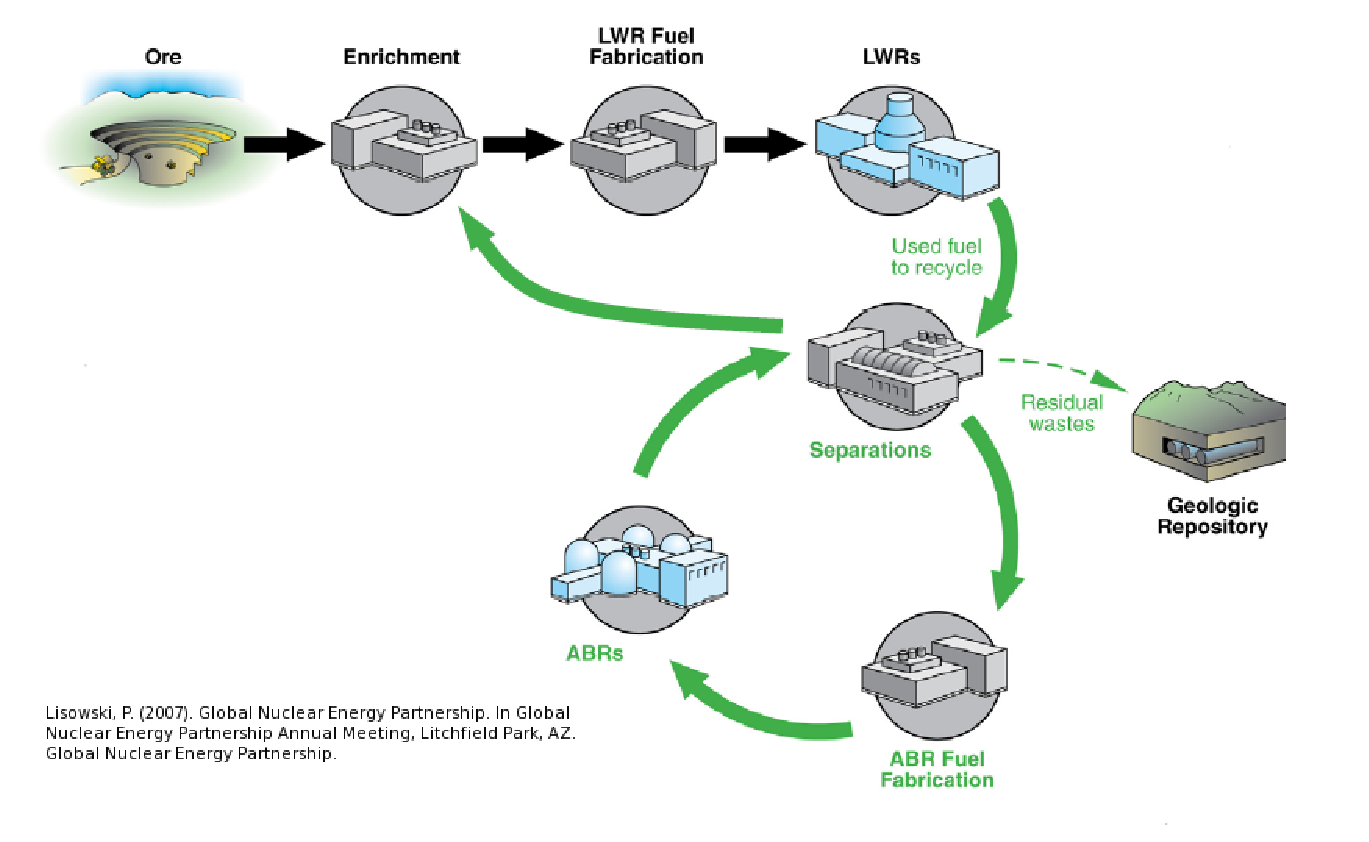
\includegraphics[height=4cm]{./images/simulations.eps}
    \end{center}
    \caption{Top level simulators are intended to model the collective 
    behavior of various fuel cycle decisions and 
    strategies \cite{lisowski_global_2007}.}
    \label{fig:simulation}
  \end{figure}
\end{frame}

\begin{frame}[ctb!]
  \frametitle{Need For an Integrated Repository Model}
  % Incorporates disposal system decisions into metrics information
  % Captures Feedbacks
  Current fuel cycle simulators neglect disposal system decisions and 
  repository behavior. Most report masses and mass indexed metrics such 
  as radiotoxicity, both meaningless without release pathway analysis
  and not informative for disposal system options.

  %        File: systools_tab.tex
%     Created: Mon Aug 29 09:00 AM 2011 C
% Last Change: Mon Aug 29 09:00 AM 2011 C
%
\begin{table}
  \centering
  \footnotesize{
  \begin{tabular}{|l|l|c|c|c|}
    \multicolumn{5}{c}{\textbf{Repository Capabilities within Systems Analysis Tools}}\\
    \hline
    Tool & Institution & Fuel Disposition & Radionuclide Transport & Heat Transport  \\
    \hline
    NUWASTE\cite{abkowitz_nuclear_2010} & NWTRB & yes & no & no \\
    VISION \cite{yacout_vision_2006} & INL   & yes & no & YMR only \\
    DANESS \cite{van_den_durpel_daness:_2006} & ANL   & no & no & no \\
    COSI   \cite{boucher_international_2010} & CEA   & yes & no & yes \\
    NFCSim \cite{schneider_nfcsim_2004} & LANL  & no & no & no \\
    CAFCA  \cite{guerin_benchmark_2009} & MIT   & no & no & no \\
    ORION  \cite{guerin_benchmark_2009} & BNL   & no & no & no \\
    TSM    \cite{turner_discrete_2010} & OCRWM & yes & no & YMR only \\
    \hline
  \end{tabular}
  \caption[System Tools]{System tools are lacking in radionuclide transport and  
  heat transport calculations in generic geolgies.}
  \label{tab:systools}
  }
\end{table}




\end{frame}


\subsection{Future Fuel Cycle Options}

\begin{frame}[ctb!]
  \frametitle{Future Fuel Cycle Options}
       % Future Fuel Cycles
    \begin{table}
      \centering
      \footnotesize{
      \begin{tabular}{|l|l|l|}
        \multicolumn{3}{c}{\textbf{Domestic Fuel Cycle Options}}\\
        \hline
        Title & Description& Challenges \\
        \hline
        \hline
        Open          & Once Through         & High Temperatures, Volumes \\
                      & Current US PWR Fleet &      \\
                      & No Separations       &      \\
                      & No Recycling         &      \\
                      & Higher Burnups &      \\
        \hline
        Modified Open & Partial Recycling    & Both high volumes and myriad fuel streams \\
                      & Next Gen. PWR Fleet &      \\
                      & Limited Separations  &      \\
                      & Limited Transmutation &      \\
                      & Advanced Fuel Forms  &      \\
                      & HLW treatment    &          \\
        \hline
        Closed        & Full Recycling       & Myriad fuel streams \\
                      & Full Separations &      \\
                      & Full Recycling &      \\
                      & VHTGR, SFRs, &      \\
                      & other transmutation & \\
                      & HLW treatment  &      \\
        \hline
      \end{tabular}
      \caption[Fuel Cycle Options]{Domestic Fuel Cycle Options }
      \label{tab:fco}
      }
    \end{table}

\end{frame}

\subsection{Geologic Disposal Concept Options}


%%----------------------------------------%%
\begin{frame}[ctb!]
  \frametitle{Repository Components}
\footnotesize{
  \begin{figure}[htbp!]
  \begin{center}
    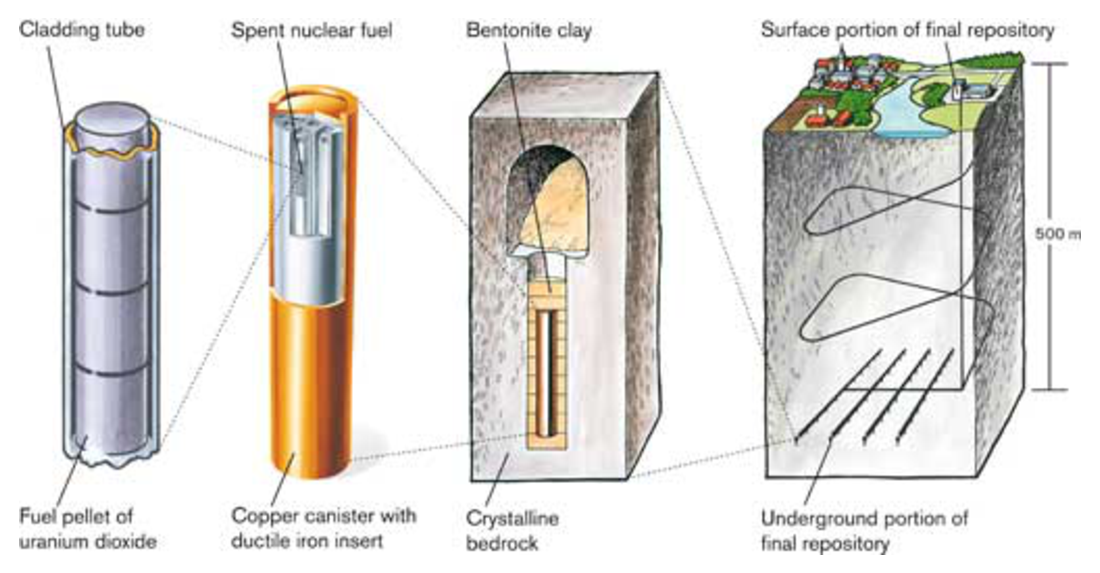
\includegraphics[width=0.7\textwidth]{./images/skb_components.eps}
  \end{center}
  \caption{Geologic disposal systems typically employ engineered barrier 
    systems as well as natural barrier systems. This is a Swedish concept in 
    granite \cite{ab_long-term_2006}.}
  \label{fig:skb_components}
\end{figure}

}
\end{frame}

%%----------------------------------------%%
\begin{frame}[ctb!]
  \frametitle{Engineered Barriers : Waste Forms}
\footnotesize{
  The first line of defense is the waste form.
  \begin{figure}[htbp!]
  \begin{center}
    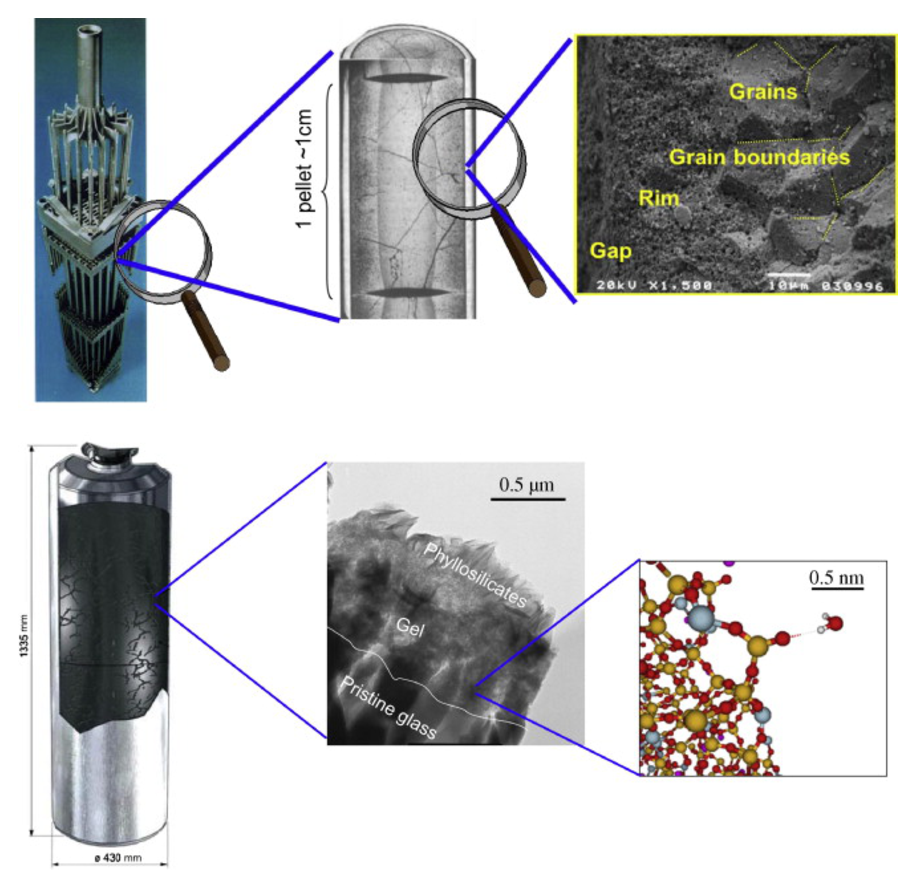
\includegraphics[width=0.5\textwidth]{./images/waste_forms_poinssot.eps}
  \end{center}
  \caption{A comparison of uranium oxide and borosilicate glass waste forms 
  \cite{poinssot_long-term_2012}.}
  \label{fig:waste_forms_poinssot}
\end{figure}

}
\end{frame}

%%----------------------------------------%%
\begin{frame}[ctb!]
  \frametitle{Engineered Barriers : Waste Packages}
\footnotesize{
  \begin{figure}[htbp!]
  \begin{center}
    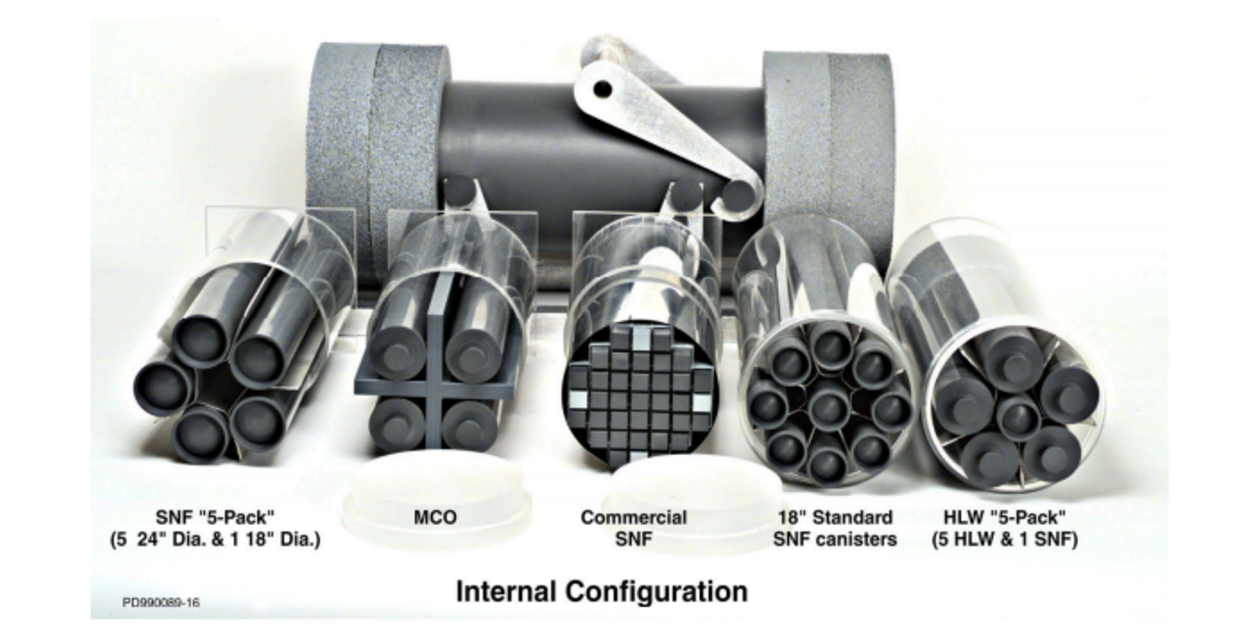
\includegraphics[width=0.7\textwidth]{./images/packages_ineel.eps}
  \end{center}
  \caption{Conceptual mockup of waste packages around waste forms 
    \cite{bridges_standardized_2001}.}
  \label{fig:packages}
\end{figure}

}
\end{frame}

%%----------------------------------------%%
\begin{frame}[ctb!]
  \frametitle{Engineered Barriers : Disposal Cask}
\footnotesize{
  \begin{figure}[htbp!]
  \begin{center}
    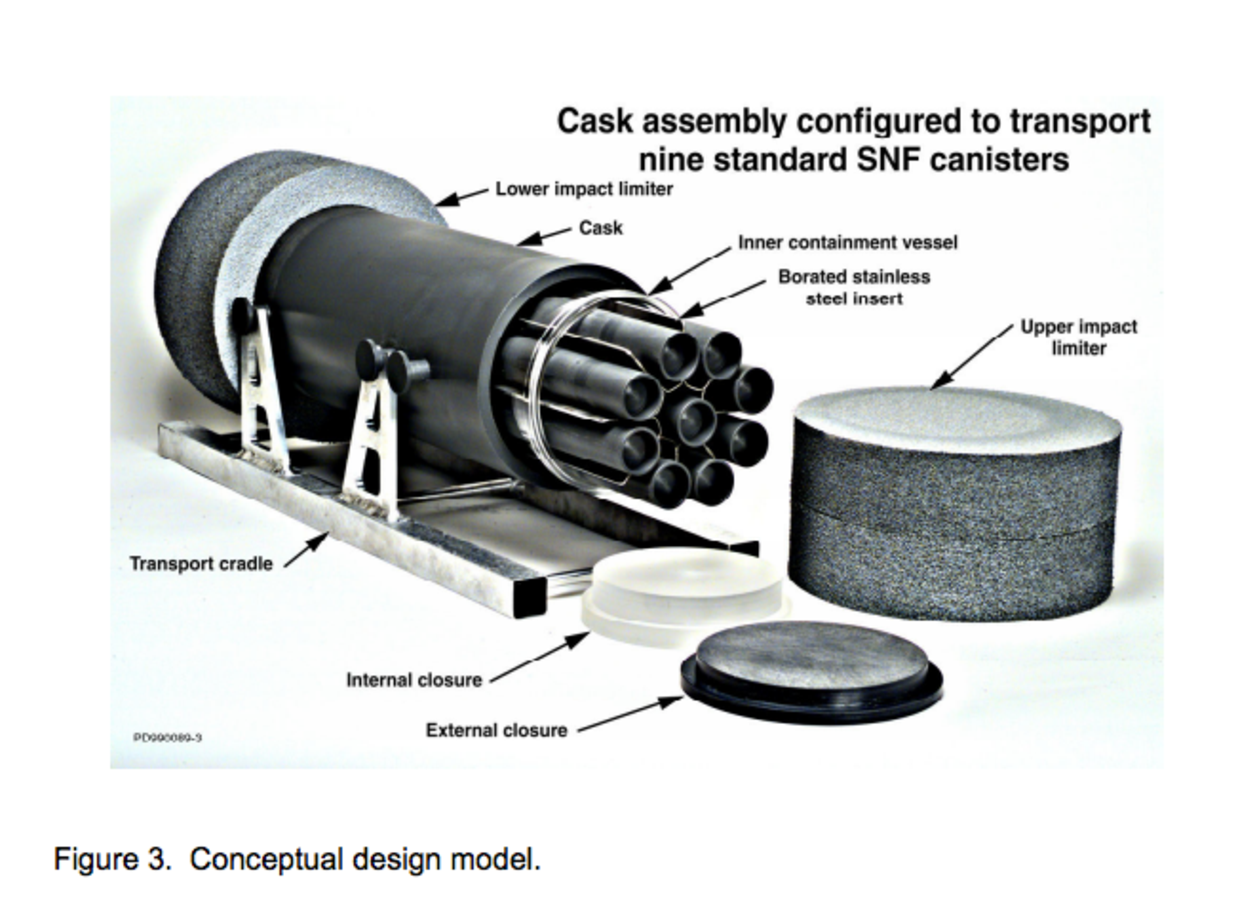
\includegraphics[width=0.7\textwidth]{./images/cask_ineel.eps}
  \end{center}
  \caption{Conceptual mockup of a transport and disposal cask 
    \cite{bridges_standardized_2001}.}
  \label{fig:packages}
\end{figure}

}
\end{frame}

%%----------------------------------------%%
\begin{frame}[ctb!]
  \frametitle{Engineered Barriers : Buffer}
\footnotesize{
  \begin{figure}[h!]
    \begin{center}
      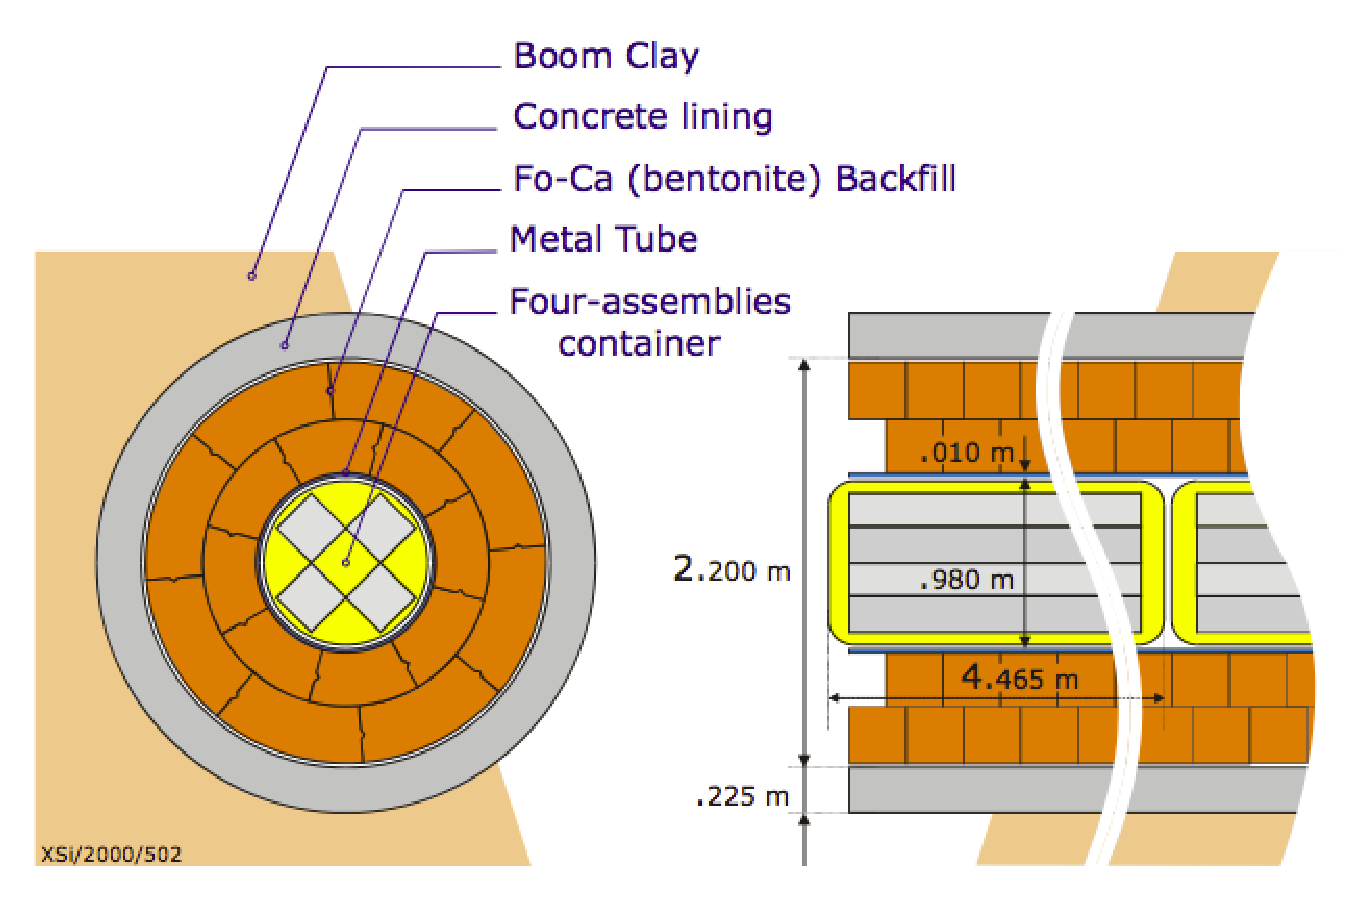
\includegraphics[height=.7\textheight]{./images/belgianClayRedImp.eps}
    \end{center}
    \caption{Belgian reference concept in Boom Clay 
    \cite{von_lensa_red-impact_2008}.}
    \label{fig:belgianClayRedImp}
  \end{figure}
}
\end{frame}

%%----------------------------------------%%
\begin{frame}[ctb!]
  \frametitle{Natural Barrier : Geology}
\footnotesize{
  \begin{figure}[htbp!]
  \begin{center}
    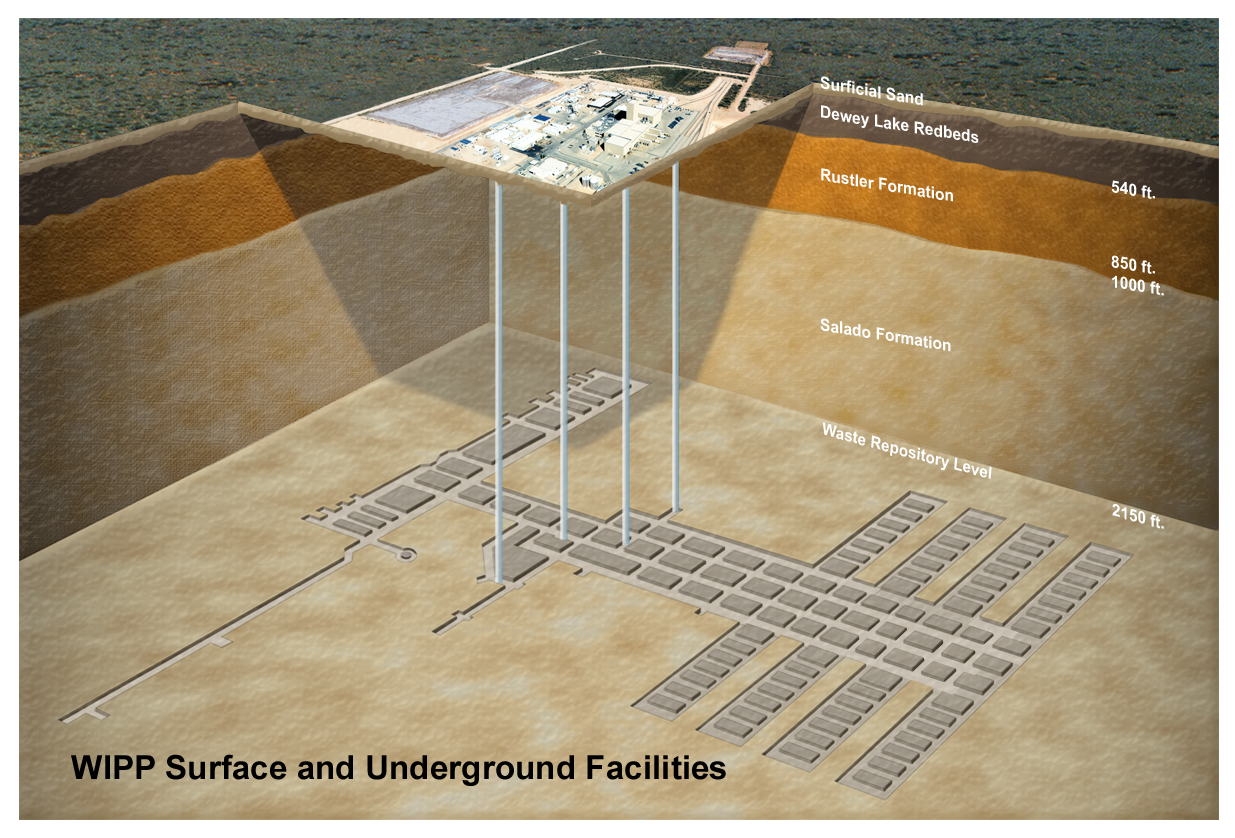
\includegraphics[width=0.7\textwidth]{./images/wipp_stratigraph.eps}
  \end{center}
  \caption{The Waste Isolation Pilot Plant has many geologic layers above the 
    salt bed \cite{doe_wipp_2013}.}
  \label{fig:wipp}
\end{figure}

}
\end{frame}

\begin{frame}
  \frametitle{Repository Layouts}

  \begin{minipage}{0.49\textwidth}
    \begin{figure}[h!]
      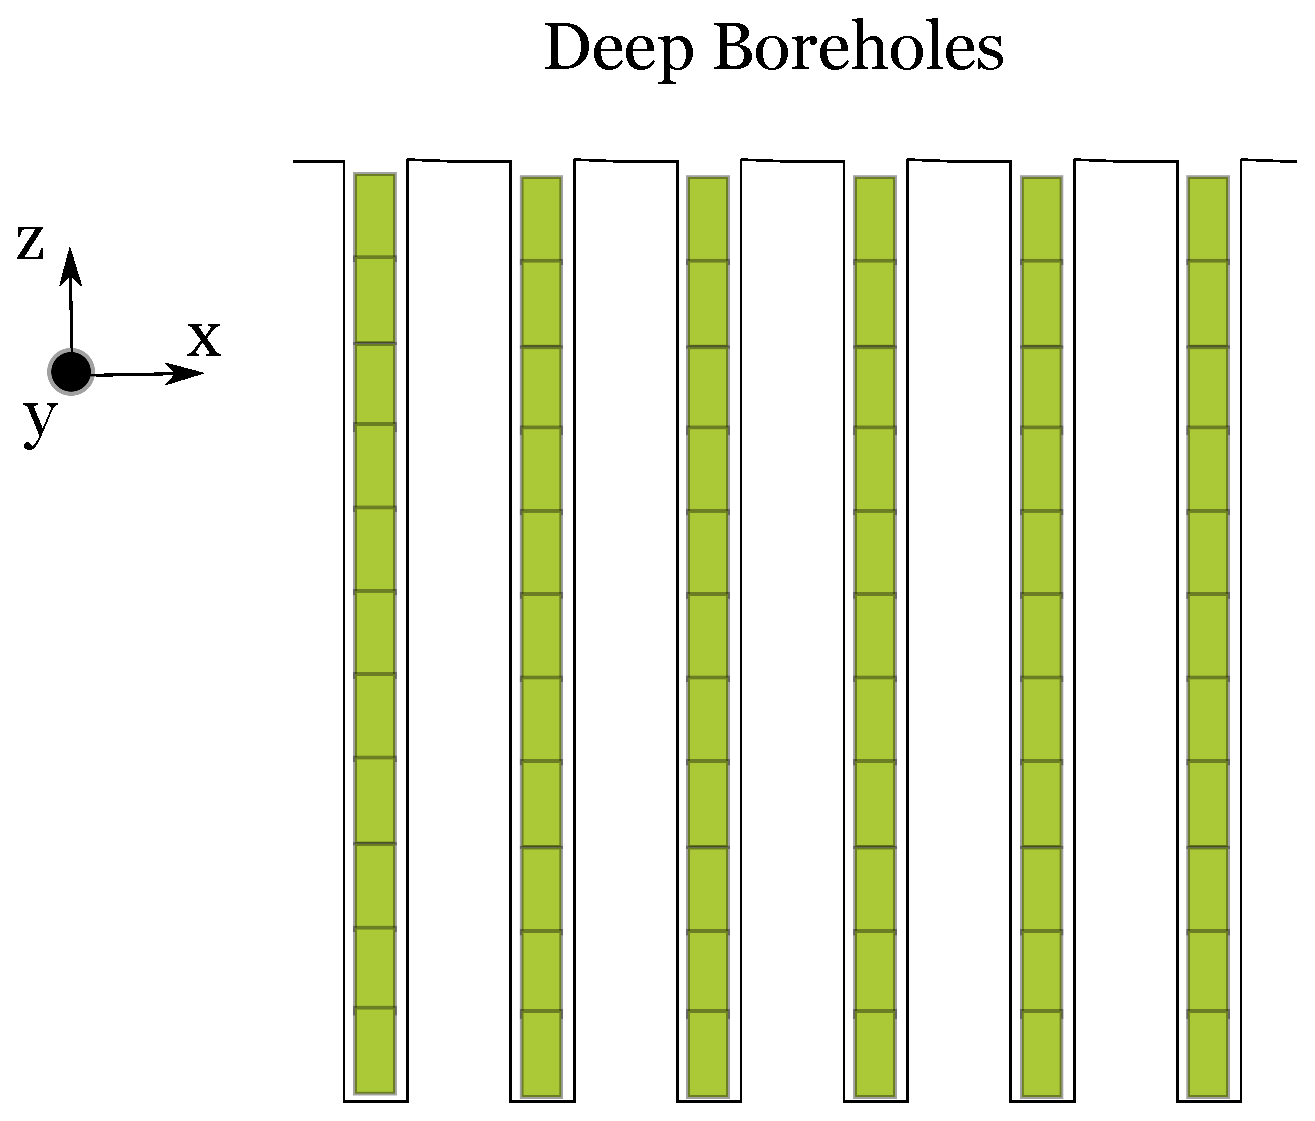
\includegraphics[width=0.75\textwidth]{./images/boreholes.eps}
    \end{figure}
    \begin{figure}[h!]
      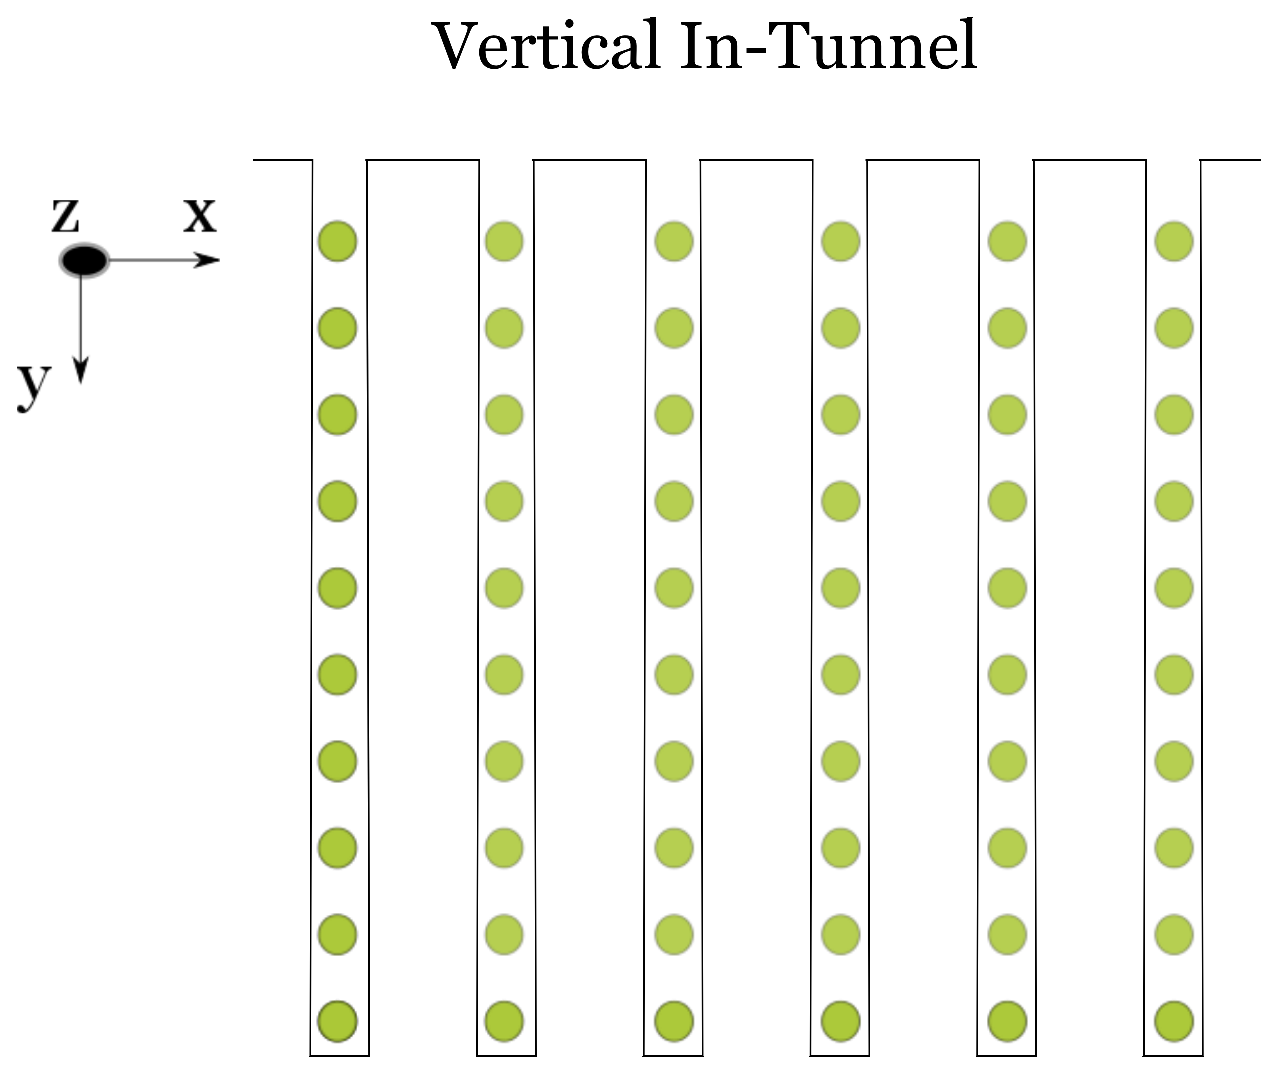
\includegraphics[width=0.75\textwidth]{./images/vertical.eps}
    \end{figure}
  \end{minipage}
  \hspace{0.01cm}
  \begin{minipage}{0.49\textwidth}
    \begin{figure}[h!]
      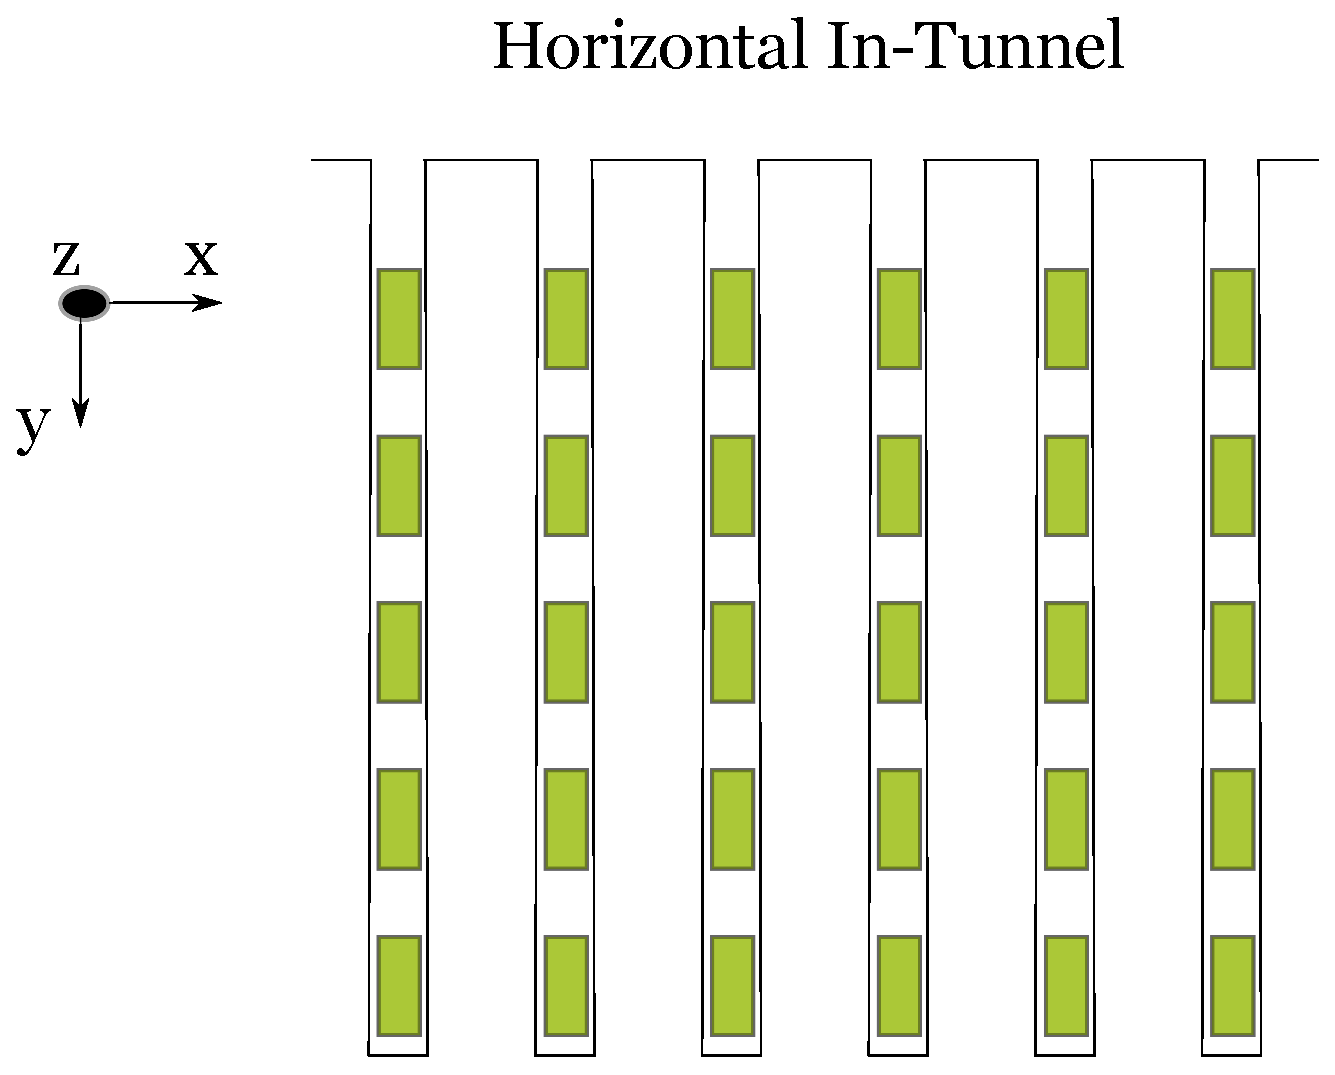
\includegraphics[width=0.8\textwidth]{./images/horizontal.eps}
    \end{figure}
    \begin{figure}[h!]
      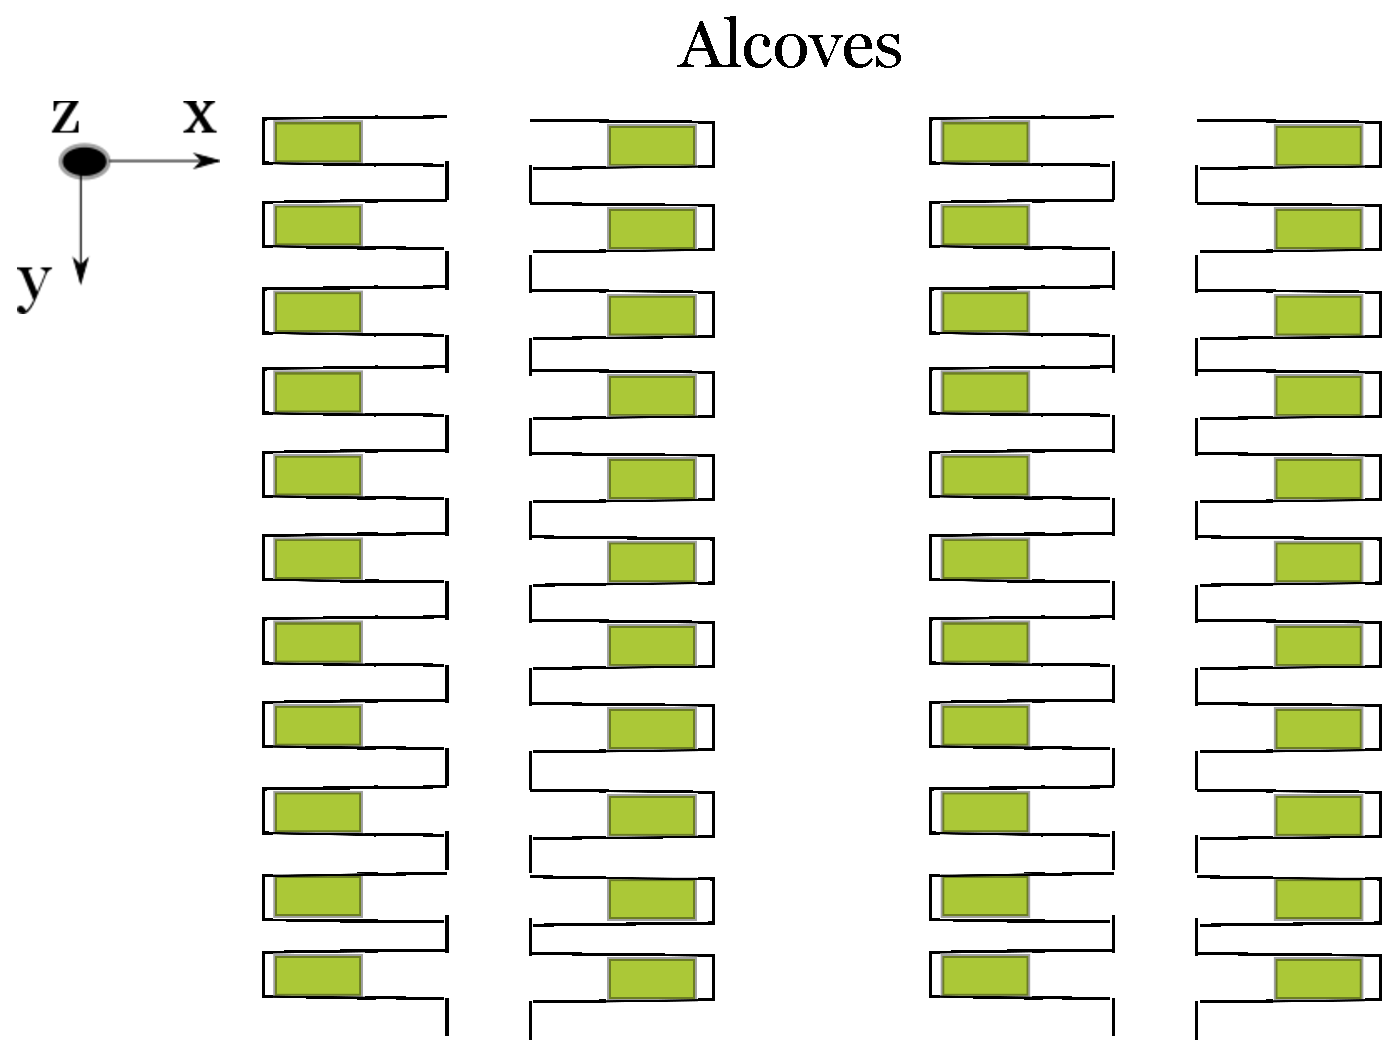
\includegraphics[width=0.8\textwidth]{./images/alcoves.eps}
    \end{figure}
  \end{minipage}

\end{frame}

\begin{frame}[ctb!]
  \footnotesize{
  \frametitle{Unsaturated, Ventilated Concepts}
  \begin{figure}[htbp!]
  \begin{center}
    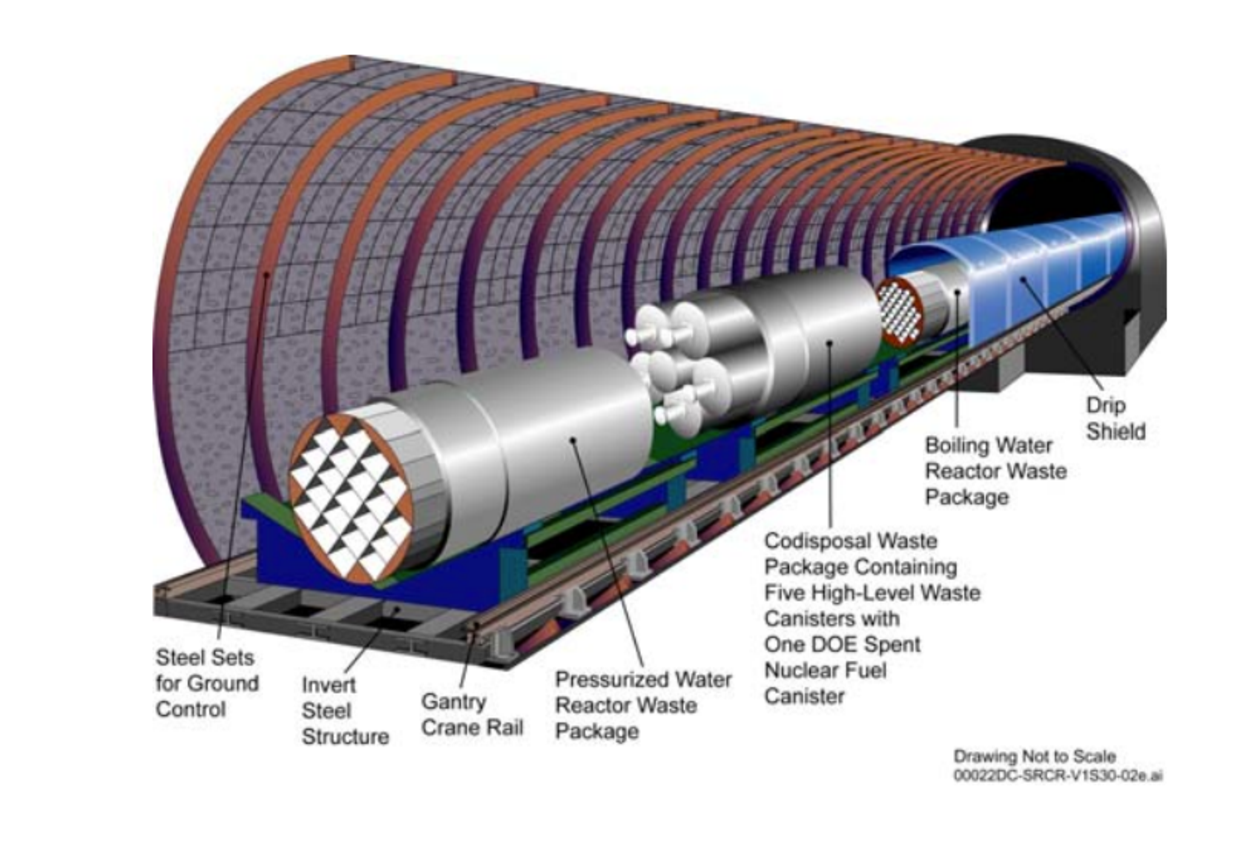
\includegraphics[height=0.7\textwidth]{./images/yucca_tunnel.eps}
  \end{center}
  \caption{The current U.S. geologic disposal concept \cite{peters_whats_2013}.}
  \label{fig:yucca_tunnel}
\end{figure}

}
\end{frame}

\begin{frame}[ctb!]
  \footnotesize{
  \frametitle{Saturated , Enclosed Concepts} 
 \begin{figure}[h!]
    \begin{center}
      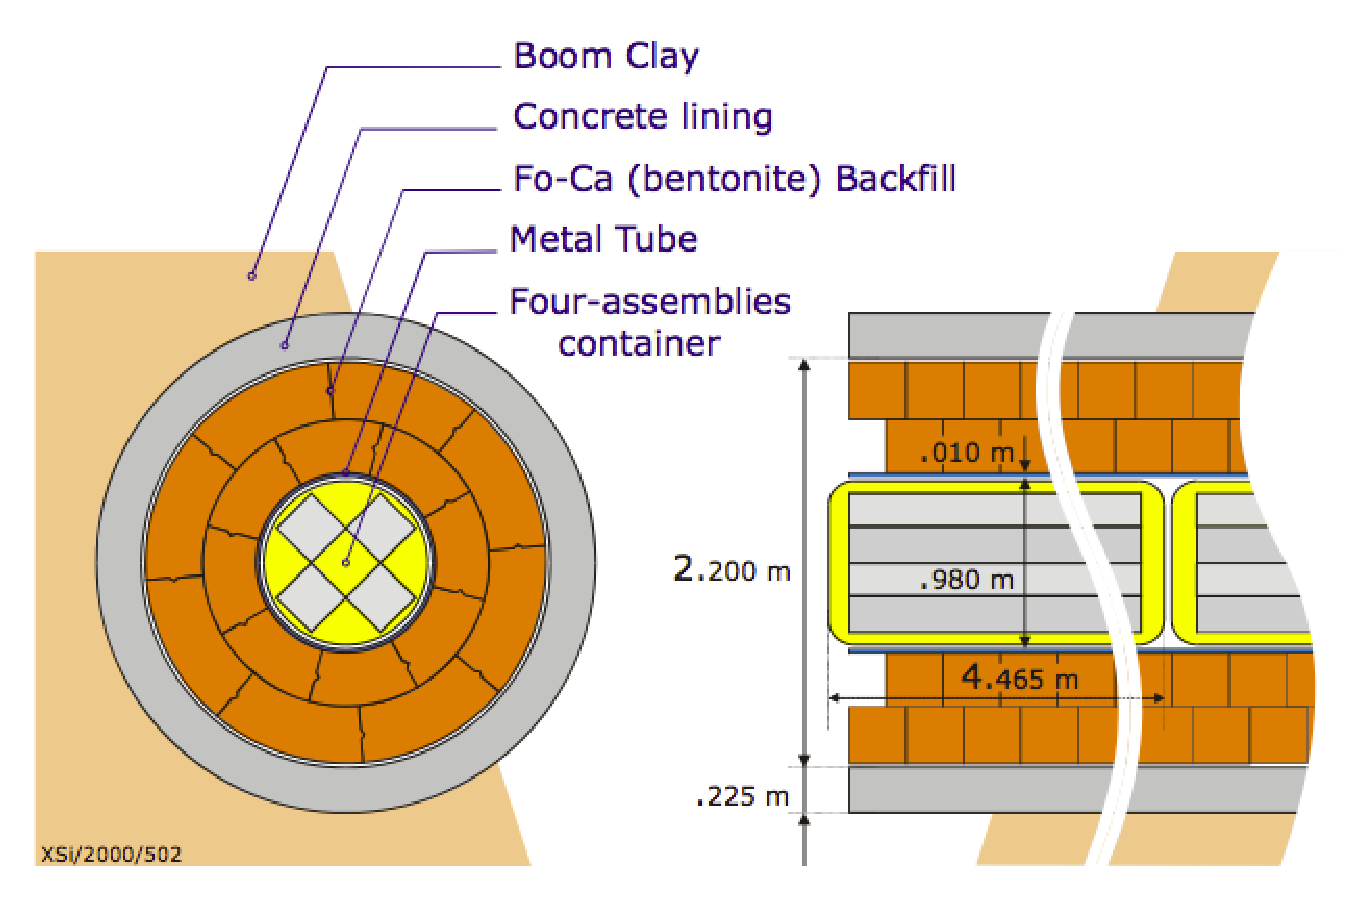
\includegraphics[height=.7\textheight]{./images/belgianClayRedImp.eps}
    \end{center}
    \caption{The Belgian reference concept in Boom Clay is backfilled very soon
   after waste emplacement without a ventilation period and is located below the water table
   \cite{von_lensa_red-impact_2008}.}
    \label{fig:belgianClayRedImp}
  \end{figure}
}
\end{frame}



\begin{frame}[ctb!]
  \frametitle{Disposal Geology Options Considered}
   \begin{minipage}{0.44\textwidth}
     \begin{figure}[h!]
         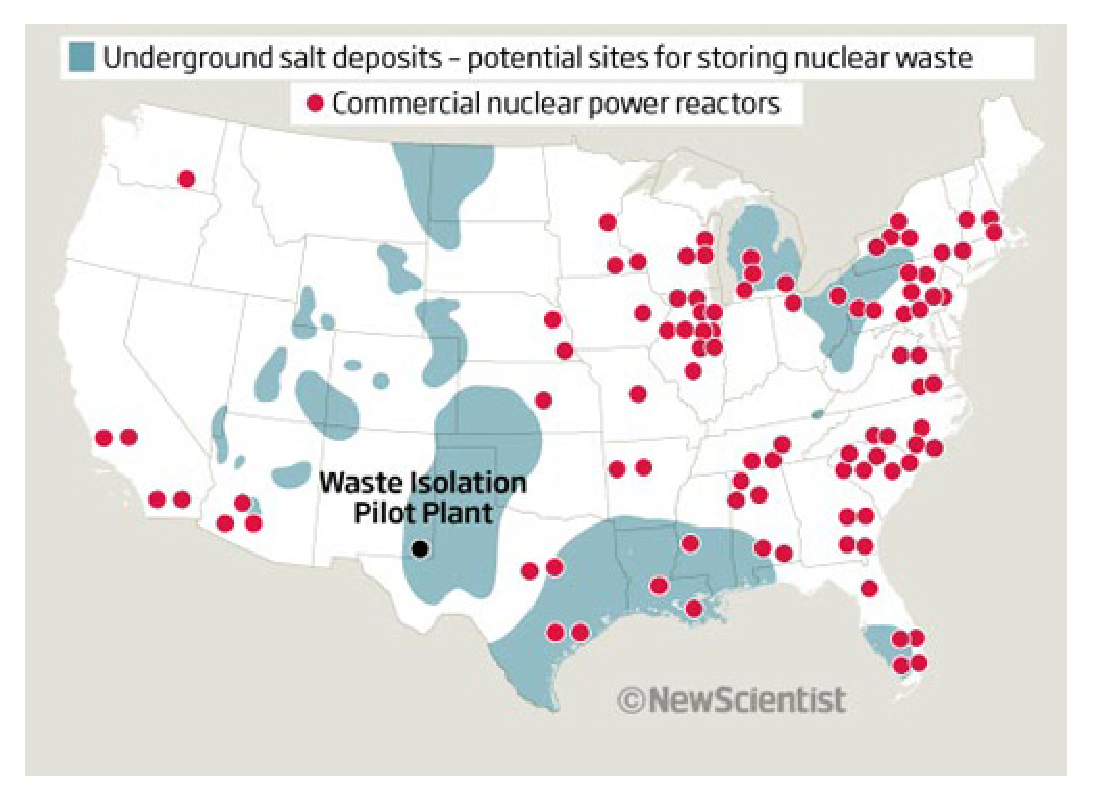
\includegraphics[width=0.7\textwidth]{./images/saltNewScientist.eps}
         \caption{U.S. Salt Deposits, ref. \cite{newscientist_where_2011}.}
     \end{figure}
     \begin{figure}[h!]
         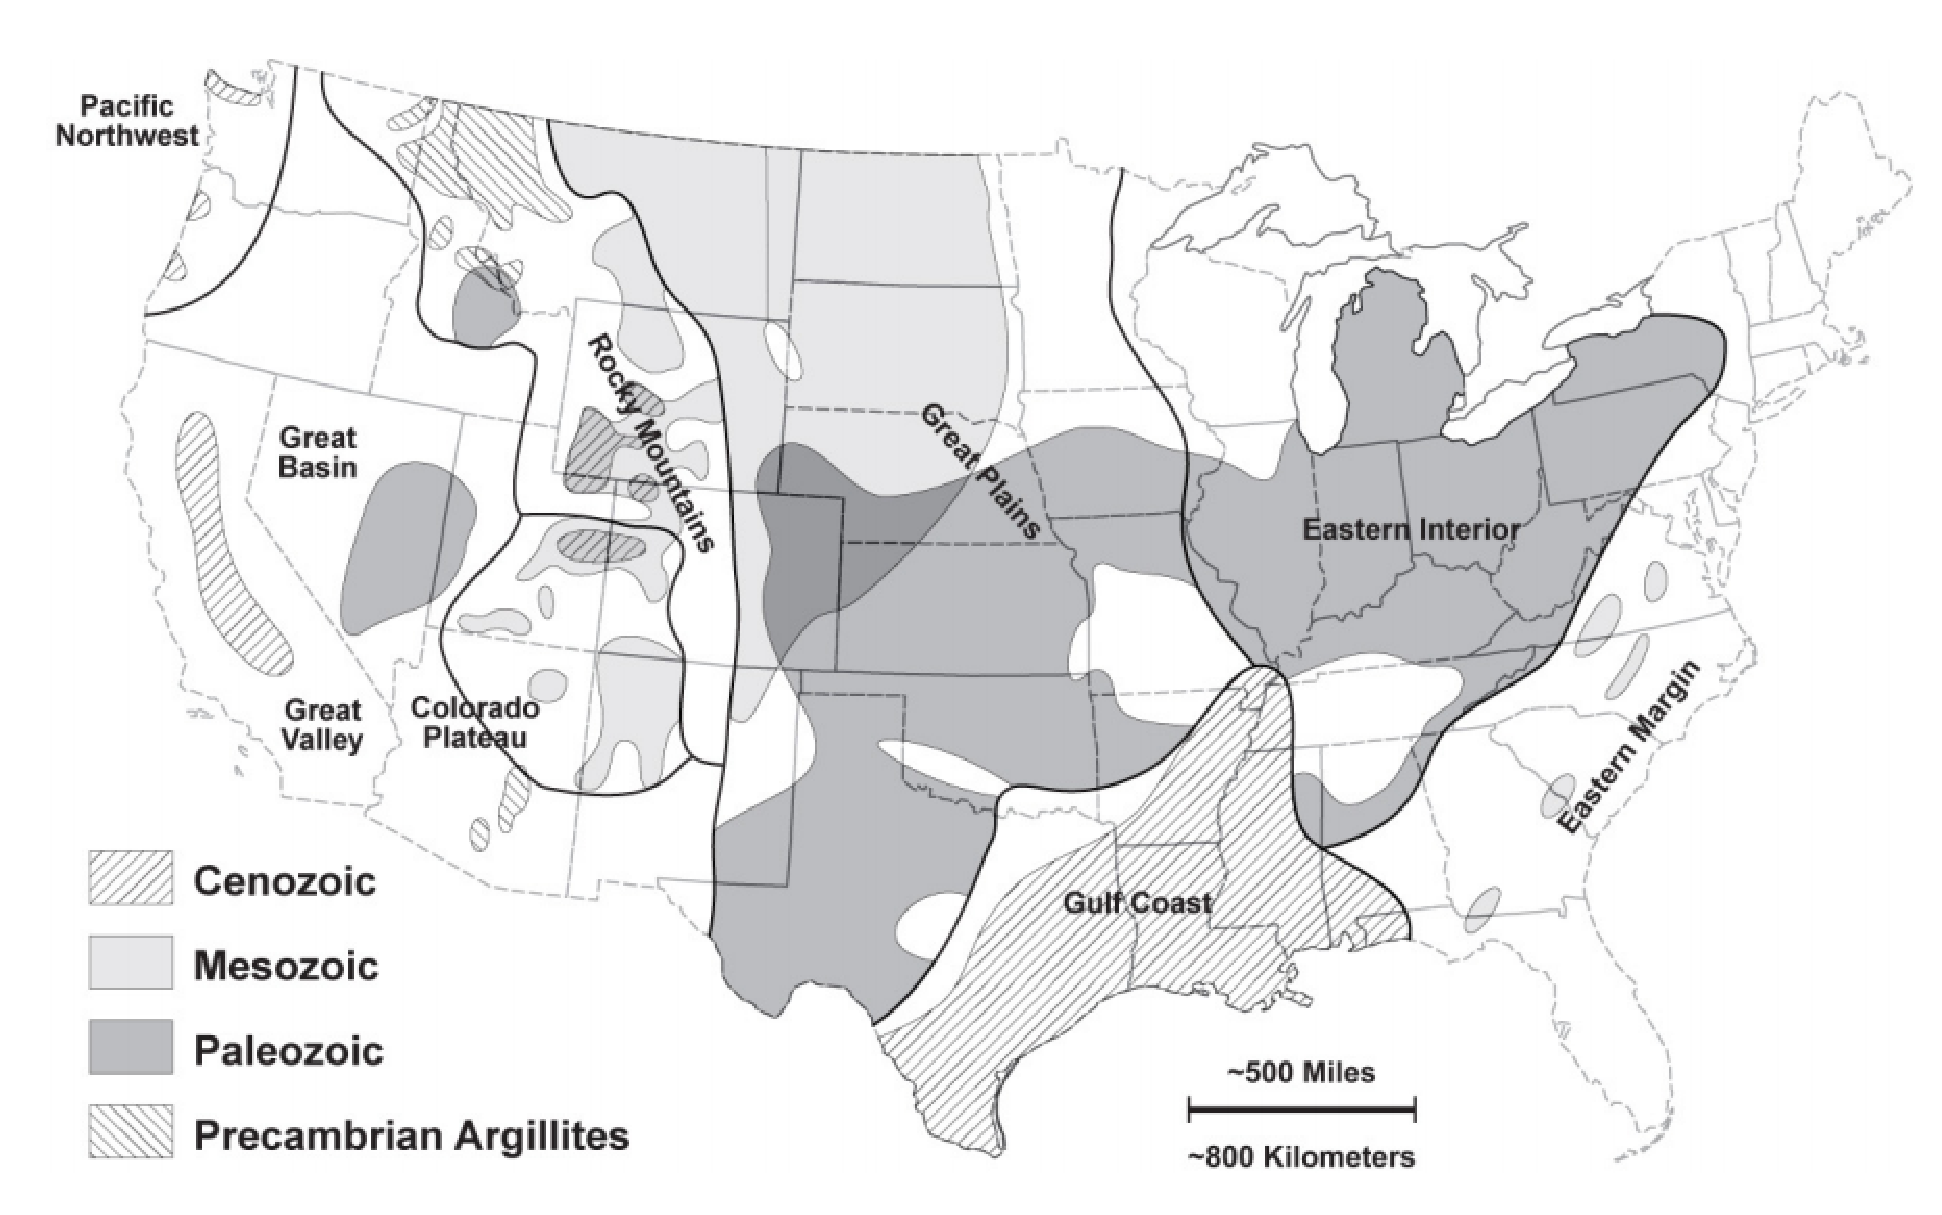
\includegraphics[width=0.7\textwidth]{./images/clayGonzales.eps}
         \caption{U.S. Clay Deposits, ref. \cite{gonzales_shales_1985}.}
     \end{figure}
   \end{minipage}
   \begin{minipage}{0.44\textwidth}
     \begin{figure}[h!]
         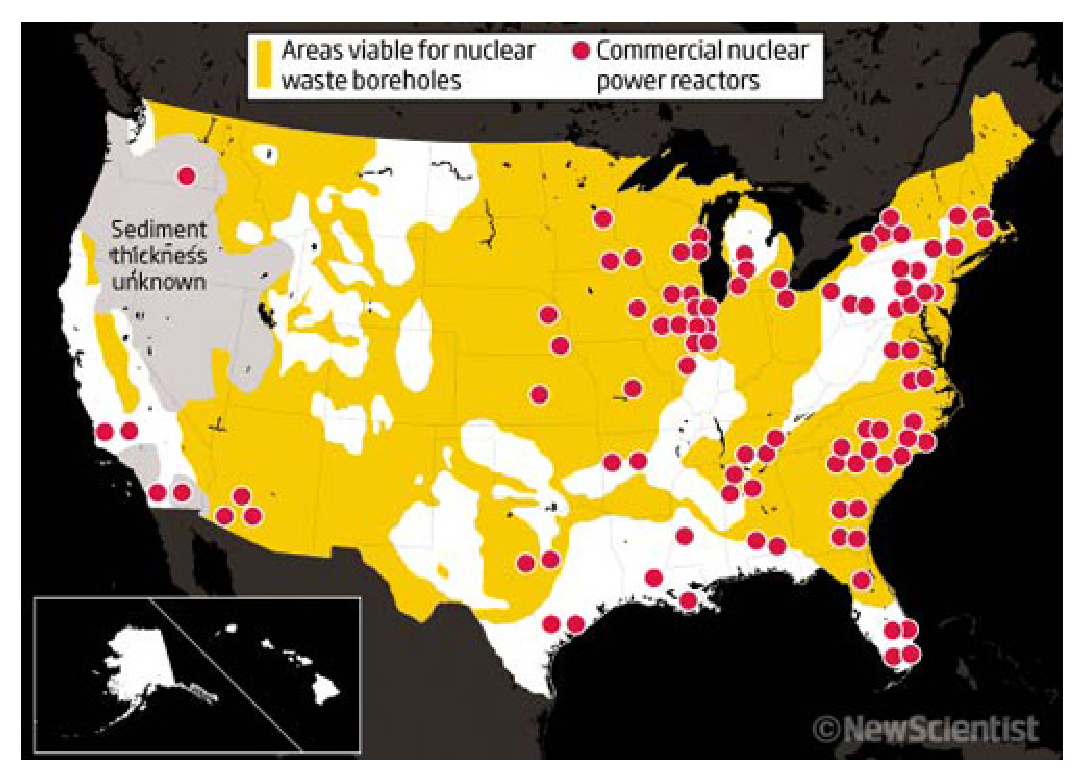
\includegraphics[width=0.7\textwidth]{./images/boreholeNewScientist.eps}
         \caption{U.S. Crystalline Basement, ref.  \cite{newscientist_where_2011}.}
     \end{figure}
     \begin{figure}[h!]
         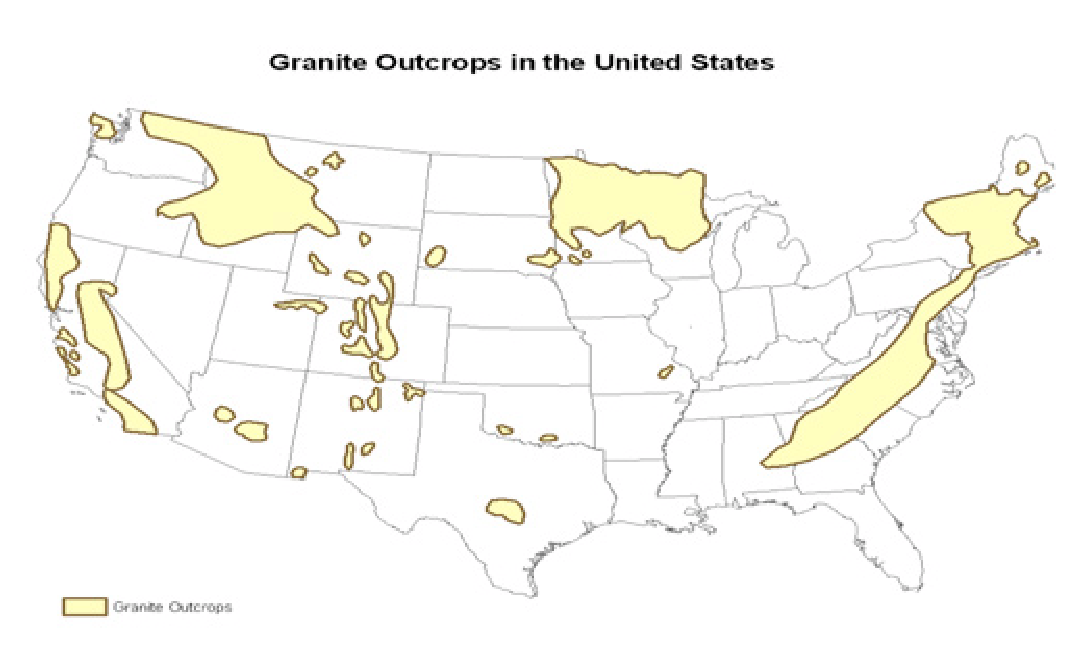
\includegraphics[width=0.7\textwidth]{./images/graniteBush.eps}
         \caption{U.S. Granite Beds, ref. \cite{bush_economic_1976}.}
     \end{figure}
   \end{minipage}
\end{frame}


\section{Modeling Paradigm}
\subsection{Cyder Overview}

\begin{frame}[ctb!]
  \frametitle{Cyder Paradigm : Modularity }
  A modular repository framework facilitates 
  \begin{itemize}
    \item  interchangable subcomponents (e.g. buffer material) so that 
      the impact on the disposal system performance may be observed
    \item and simulations with varying levels of detail.
  \end{itemize}
 \pause
  Integration with a fuel cycle simulator facilitates
  \begin{itemize}
    \item analysis of feedback effects upon the fuel cycle
    \item and investigation of fuel cycle choices on disposal system 
      performance.
  \end{itemize}
\end{frame}


\begin{frame}[ctb!]
  \frametitle{Cyder Paradigm : Waste Stream Acceptance}
  \footnotesize{
  
To participate in fuel cycle simulation, the repository model must accept arbitrary 
spent fuel and high level waste streams. A waste stream is a material data 
object resulting from the Cyclus simulated fuel cycle.  
  \begin{figure}[htbp!]
    \begin{center}
      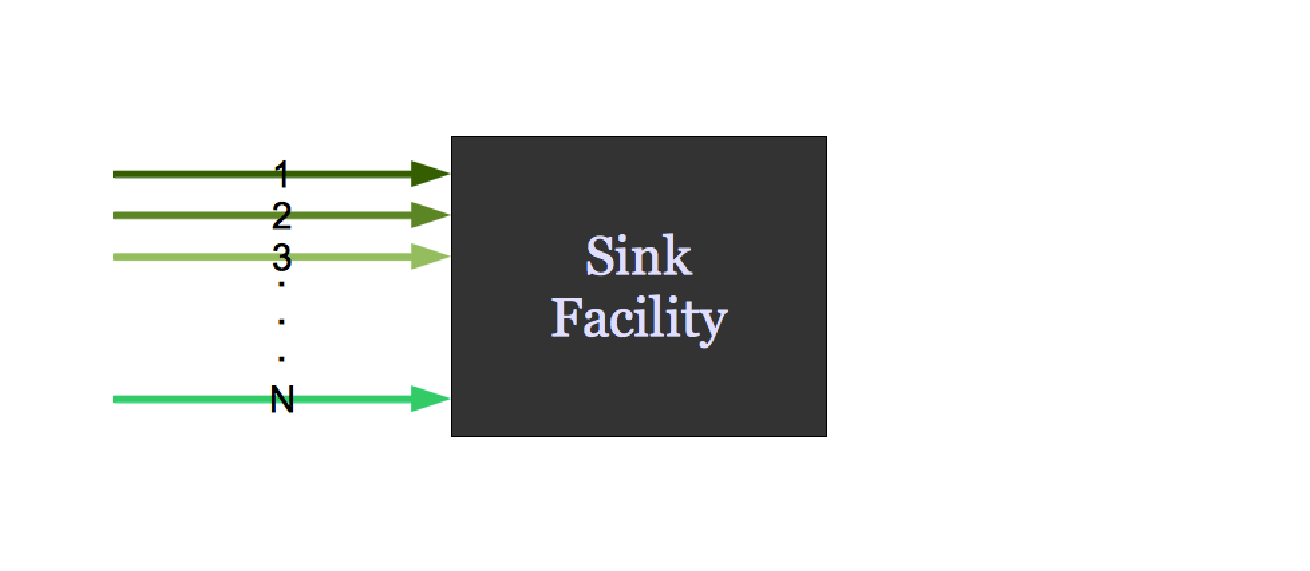
\includegraphics[height=5cm]{./images/sinkfacility.eps}
    \end{center}
    \caption{ The Cyder Facility dynamically accepts material from the 
    coupled fuel cycle simulation.} 
    \label{fig:sinkfacility}
  \end{figure}
% Sink Facility ?
}
\end{frame}

\begin{frame}[ctb!]
  \frametitle{Cyder Paradigm : Waste Stream Conditioning}
  \footnotesize{

    \textbf{Waste conditioning} is the process of packing a waste stream into an appropriate 
waste form.  The Cyder model loads discrete waste forms with discrete waste 
stream contaminant vectors as depicted in Figure \ref{fig:ws_conditioning}.
  
\begin{figure}[htbp!]
\begin{center}
\def\svgwidth{.5\textwidth}
\input{./images/ws_conditioning.eps_tex}
\end{center}
\caption{Waste streams are conditioned into the appropriate waste form 
according to user-specified pairings.}
\label{fig:ws_conditioning}
\end{figure}
}
\end{frame}

\begin{frame}[ctb!]
  \frametitle{Cyder Paradigm : Waste Form Packaging}
  \footnotesize{

    \textbf{Waste packaging} is the process of placing one or many waste forms into a 
containment package. Once the waste stream has been conditioned into a waste 
form, that waste form Component is loaded into a waste package Component as 
depicted in Figure \ref{fig:wf_packaging}.  

\begin{figure}[htbp!]
\begin{center}
\def\svgwidth{.5\textwidth}
\input{./images/wf_packaging.eps_tex}
\end{center}
\caption{Waste forms are loaded into the appropriate waste package 
according to user-specified pairings.}
\label{fig:wf_packaging}
\end{figure}
}
\end{frame}

\begin{frame}[ctb!]
  \frametitle{Cyder Paradigm : Waste Package Emplacement}
\footnotesize{
  \begin{columns}[c]
    \column{0.3\linewidth}
Finally, the waste package is \textbf{emplaced} in a buffer component, which 
contains many other waste packages, spaced evenly in a grid. The grid is 
defined by the user input and depends on repository depth, $\Delta z$, waste 
package spacing, $\Delta x$, and tunnel spacing, $\Delta y$ as in Figure 
\ref{fig:repo_layout}.

    \column{0.6\linewidth}
\begin{figure}[htbp!]
\begin{center}
\def\svgwidth{.5\textwidth}
\input{./images/repo_layout.eps_tex}
\end{center}
\caption{The repository layout has a depth and a uniform package spacing.}
\label{fig:repo_layout}
\end{figure}
\end{columns}
  }
\end{frame}


\begin{frame}
  \frametitle{Nested Components}
  Each Component has : 
  \begin{itemize}
    \item a Geometry to describe its dimensions and location
    \item a NuclideModel for contaminant transport 
    \item a ThermalModel for heat transport
    \item a Parent Component at its external barrier
    \item one or more Daughter Components at its internal barrier
  \end{itemize}

  Components have other data members such as a Type (WF, WP, BUFFER, FF), a 
  material data table, a start date, etc. 
\end{frame}

\begin{frame}
  \frametitle{Nested Components}
  The NuclideModel in a Component can be interchangeably represented by any of 
  the four nuclide transport models. 
    \begin{itemize}
      \item Degradation Rate Based Failure Model
      \item Mixed Cell with Degradation, Sorption, Solubility Limitation
      \item Lumped Parameter Model
      \item 1D Advection Dispersion Solution
    \end{itemize}
\end{frame}


%\subsection{Cyder Models}
%\input{paradigm_models}
%\subsection{Cyder Data}
%\input{paradigm_data}

%\section{Abstraction Methodology}
%

\begin{frame}[ctb!]
  \frametitle{Abstraction Methodology}
\footnotesize{
describe abstraction - thermal, radionuclide transport tools, sensitivity experiments, etc.

}
\end{frame}

\begin{frame}[ctb!]
  \frametitle{Abstraction Methodology}
\footnotesize{
abstraction methodology cont'd
}
\end{frame}

\subsection{Thermal Transport in Cyder}
\begin{frame}[ctb!]
\frametitle{Thermal Modeling in Cyder}
Two types of thermal modeling occur in Cyder. 
\begin{itemize}
\item The first is \textbf{capacity estimation} for waste stream acceptance.
\item The next is \textbf{heat evolution} which (optionally) determines heat evolution in 
the modules over repository lifetime.
\end{itemize}
\pause
Each can be acheived with one thermal model,
\begin{itemize}
\item This model employs a Specific Temperature Change algorithm \cite{radel_effect_2007, radel_repository_2007} and
\item relies on a supporting \textbf{response database} combining detailed 
spent nuclear fuel composition data \cite{carter_fuel_2011} with a detailed 
thermal repository performance analysis tool from Lawrence Livermore National 
Lab (LLNL) and the Used Fuel Disposition (UFD) 
campaign \cite{greenberg_application_2012}.  
\item This method is capable of rapid estimation of temperature increase near emplacement tunnels as a function of 
\begin{itemize}
\item waste composition,
\item limiting radius, $r_{lim}$, 
\item waste package spacing, $S$, 
\item near field thermal conductivity, $K_{th}$, 
\item and near field thermal diffusivity, $\alpha_{th}$.
\end{itemize}
\end{itemize}
\end{frame}




\subsection{Specific Temperature Change Method}
Introduced by Radel, Wilson et al., the \gls{STC} method uses 
a linear approximation to arrive at the thermal loading density limit 
\cite{radel_repository_2007, radel_effect_2007}.  
Since the thermal response in a system with a long term transient response is strong function of the 
transient decay power, it is also a strong function of the isotopic 
composition of the waste. Thus, the time dependent temperature change, $\Delta 
T$, at the limiting radius, $r_{lim}$, can be approximated as proportional to the 
mass loading density. First, $\Delta T$ is determined for a limiting loading density 
of the particular material composition then it is normalized to a single 
kilogram of that material, $\Delta t$, the so called \gls{STC}. 

\begin{align}
 \Delta T(r_{lim}) &= m \cdot \Delta t(r_{lim})
 \label{STC}
 \intertext{where}
 \Delta T &= \mbox{ Temperature change due to m }[K]\nonumber\\
 m &= \mbox{ Mass of heat generating material }[kg]\nonumber \\
 \Delta t &= \mbox{ Temperature change due to 1 kg }[K]\nonumber\\
 r_{lim} &= \mbox{ Limiting radius } [m].\nonumber
\end{align}

For an arbitrary waste stream composition, scaled curves, $\Delta t_i$, calculated in this 
manner for individual isotopes can be superimposed for each isotope to arrive at an 
approximate total temperature change.

\begin{align}
 \Delta T (r_{lim}) &\sim \sum_{i} m_i \Delta t_i(r_{lim})
 \label{superposition}
\intertext{where}
 i &= \mbox{ An isotope in the material } [-]\nonumber\\
 m_i &= \mbox{ mass of isotope i  } [kg]\nonumber\\
 \Delta t_i &= \mbox{ Specifc temperature change due to \textsl{i} } [K].\nonumber
\end{align}



\subsection{Supporting Thermal Response Dataset}
To support this calculation in \Cyder, a reference data set of temperature change 
curves was calculated. Repeated runs of a detailed analytic model over the range of values in Table 
\ref{tab:thermal_cases} determined \gls{STC} values over a range of thermal 
heat limit radii, $r_{lim}$, thermal diffusivity values, $\alpha_{th}$,
thermal conductivity values, $K_{th}$ and waste package spacings, $S$. Linear 
interpolation across the discrete parameter space provides a simple thermal 
reference dataset for use in \Cyder.

\begin{table}[ht!]
\centering
\footnotesize{
\begin{tabular}{|l|l|l|r|}
\multicolumn{4}{c}{\textbf{Thermal Cases}}\\
\hline
\textbf{Parameter} & \textbf{Symbol} & \textbf{Units} & \textbf{Value Range} \\
\hline
Diffusivity & $\alpha_{th}$ & $[m^2\cdot s^{-1}]$ & $1.0\times10^{-7}-3.0\times10^{-6}$\\
\hline
Conductivity & $K_{th}$     & $[W\cdot m^{-1} \cdot K^{-1}]$ & $0.1 - 4.5$ \\
\hline
Spacing & $S$ & $[m]$ & 2, 5, 10, 15, 20, 25, 50 \\
\hline
Radius & $r_{lim}$ & $[m]$ & 0.1, 0.25, 0.5, 1, 2, 5 \\
\hline
Isotope & $i$ & $[-]$ & $^{241,243}Am,$  \\
        & & & $^{242,243,244,245,246}Cm,$  \\
        & & & $^{238,240,241,242}Pu$  \\
        & & & $^{134,135,137}Cs$  \\
        & & & $^{90}Sr$  \\
\hline
\end{tabular}
\caption{A thermal reference dataset of \gls{STC} values as a function of each of these parameters was generated by repeated parameterized runs of the LLNL 
MathCAD model\cite{greenberg_application_2012, greenberg_investigations_2012}.}
\label{tab:thermal_cases}
}
\end{table}



The analytic model used to populate the reference dataset was created at 
\gls{LLNL} for the \gls{UFD} campaign. In this tool, heat limited thermal 
response is calculated analytically for each geologic medium, for many waste package 
loading densities, and for many fuel cycle options \cite{hardin_generic_2011, 
greenberg_investigations_2012, greenberg_application_2012}. It employs an 
analytic model from Carslaw and Jaeger and is implemented in MathCAD 
\cite{carslaw_conduction_1959, ptc_mathcad_2010}.  The integral solver in the 
MathCAD toolset is the primary calculation engine for the analytic MathCAD 
thermal model, which relies on superposition of point, finite-line, and line 
source integral solutions.  

%The transient state of the temperature at the calculation radius is found with a convolution of the transient far field solution with the steady state near field solution.  The process is then iterated with a one year resolution in order to arrive at a temperature evolution over the lifetime of the repository. 
%
%In a two dimensional grid of waste packages, the central package is represented by the finite line solution

Figure \ref{fig:CmScaling} demonstrates the scaling of an STC curve according to 
equation \eqref{STC} to represent the heat from $25.9g$ of initial $^{242}Cm$ using 
the reference data set. 

\begin{figure}[h!]
\begin{center}
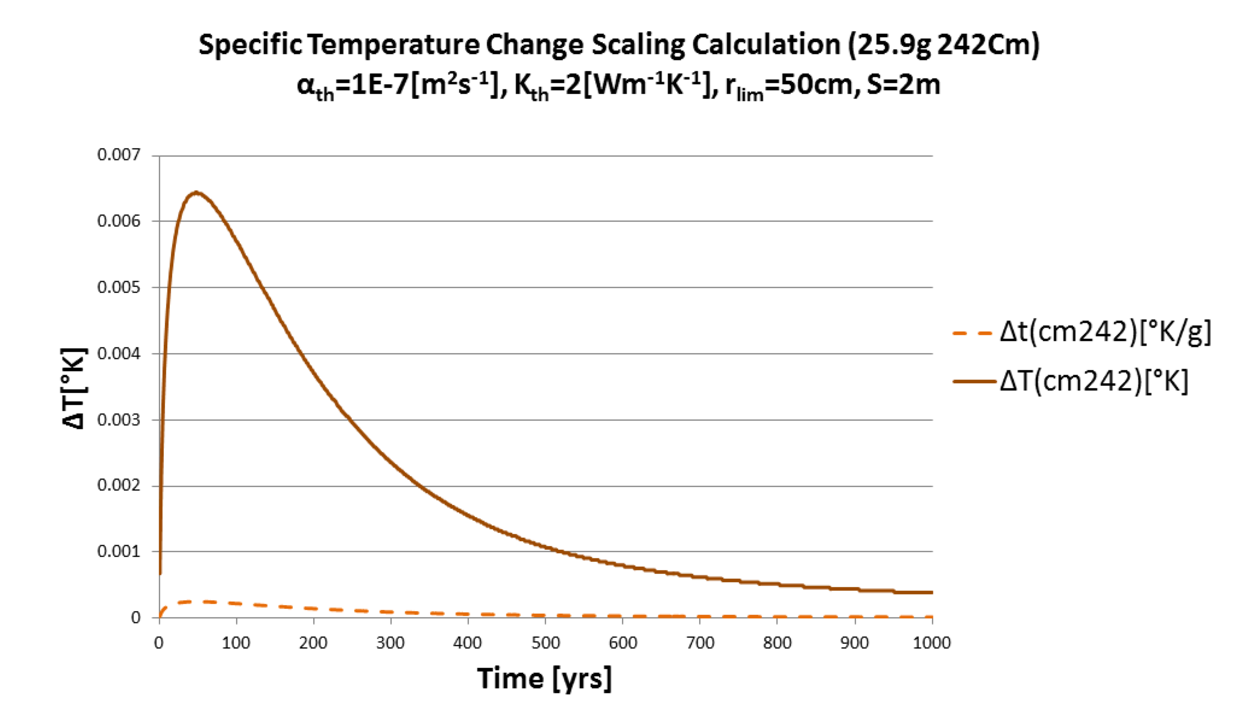
\includegraphics[width=\columnwidth]{./chapters/methodology/thermal_models/CmScaling.eps}
\end{center}
\caption[Scaling of and STC curve for $^{242}Cm$]{As a demonstration of the calculation procedure, the temperature change 
  curve for one initial gram of $^{242}Cm$ and is scaled to represent $25.9g$, 
  approximately the $^{242}Cm$ inventory per MTHM in 51GWd burnup UOX PWR fuel. }
\label{fig:CmScaling}
\end{figure}


The supporting database was limited to some primary heat contributing isotopes 
present in traditional spent nuclear fuel, $H$, 
such that the superposition in equation \eqref{superposition} becomes 

\begin{align}
\Delta T (r_{lim},S,K_{th},\alpha_{th})&\sim \sum_{i\in H} m_i \Delta t_i(r_{lim},S,K_{th},\alpha_{th})
\label{superposition_approx}
\intertext{where}
H &= \mbox{ set of high heat isotopes }[-]\nonumber\\
S &= \mbox{ uniform waste package spacing } [m]\nonumber\\
K_{th} &= \mbox{ thermal conductivity } [W\cdot m^{-1}\cdot K^{-1}]\nonumber\\
\alpha_{th} &= \mbox{ thermal diffusivity } [m^2\cdot s^{-1}]\nonumber\\
\end{align}

The use of this superposition is demonstrated in Figure 
\ref{fig:CmSuperposition}.

\begin{figure}[ht!]
\begin{center}
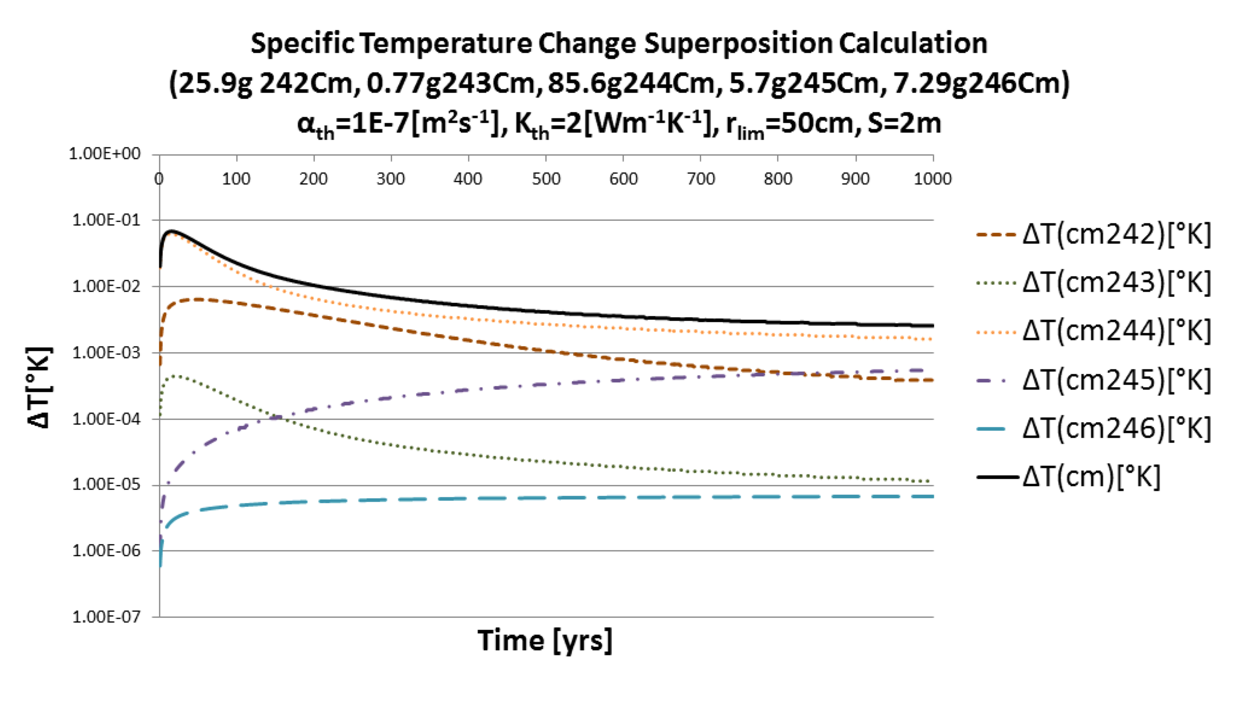
\includegraphics[width=\columnwidth]{./chapters/methodology/thermal_models/CmSuperposition.eps}
\end{center}
\caption[Superposition of scaled Cm STC curves]{As a demonstration of the calculation procedure, scaled temperature change 
  curves for five curium isotopes are superimposed to achieve a total temperature 
change (note log scale).}
\label{fig:CmSuperposition}
\end{figure}

%\begin{align}
%  T_{line}(t,x,y,z) &= \frac{1}{8\pi K_{th}} 
%  \bigintsss_0^t\!\frac{q_L(t')}{t-t'}e^{ \frac{-\left(x^2 + z^2\right)}{4\alpha 
%  (t-t')} }\nonumber\\ &\cdot\left[ \erf{\left[ \frac{1}{2} \frac{\left( y + 
%  \frac{L}{2} \right)}{\sqrt{\alpha(t-t')}}  \right]} - \erf{\left[ \frac{1}{2} 
%  \frac{\left( y - \frac{L}{2} \right)}{\sqrt{\alpha(t-t')}}  \right]} 
%  \right]\,\mathrm{dt'},
%  \label{line}
%  \intertext{adjacent packages within the central tunnel are represented by the 
%  point source solution }
%  T_{point}(t,r) &= 
%  \frac{1}{8K_{th}\sqrt{\alpha}\pi^{\frac{3}{2}}}\bigintsss_0^{-t}\!\frac{q(t')}{(t-t')^{\frac{3}{2}}}e^{\frac{-r^2}{4\alpha(t-t')}}\,\mathrm{dt'},
%  \label{point}
%  \intertext{and adjacent disposal tunnels are represented by infinite line 
%  source solutions}
%  T_{\infty line}(t,x,z) &= \frac{1}{4\pi K_{th}} 
%  \bigintsss_0^t\!\frac{q_L(t')}{t-t'}e^{ \frac{-\left(x^2 + z^2\right)}{4\alpha 
%  (t-t')} }
%  \intertext{in infinite homogeneous media, where}
%  \label{infline}
%  \alpha &= ~~\mbox{thermal diffusivity } [m^2\cdot s^{-1}]\nonumber\\
%  q(t) &= ~~\mbox{point heat source} [W]\nonumber\\
%  \intertext{and}
%  q_L(t) &= ~~\mbox{linear heat source} [W\cdot m^{-1}]\nonumber
%\end{align}
%Superimposed point and line source solutions allow for a notion of the 
%repository layout to be modeled in the host rock.


\subsection{Radionuclide Transport in Cyder}

\begin{frame}
  \frametitle{Nested Components}
  The NuclideModel in a Component can be interchangeably represented by any of 
  the four nuclide transport models. 
    \begin{itemize}
      \item Degradation Rate Based Failure Model
      \item Mixed Cell with Degradation, Sorption, Solubility Limitation
      \item Lumped Parameter Model
      \item 1D van Genuchten Advection Dispersion Solution
    \end{itemize}
\end{frame}

\begin{frame}
\frametitle{Clay GDSM Model}
\begin{figure}[htbp!]
  \begin{center}
    \includegraphics[width=0.9\textwidth]{./images/clay_gdsm.eps}
  \end{center}
  \caption{The Clay Generic Disposal System Model (GDSM) was used for 
  preliminary sensitivity analysis, abstraction iteration, and validation.
  This figure was reproduced from Figure 3.3-2 in \cite{clayton_generic_2011}.}
  \label{fig:clay_gdsm}
\end{figure}

\end{frame}

\begin{frame}
  \frametitle{Advection Dispersion Equation}
  \footnotesize{
    In a saturated, reducing environment, contaminants are transported by 
    \textbf{dispersion} and \textbf{advection} 
    \cite{schwartz_fundamentals_2004, 
    wang_introduction_1982, van_genuchten_analytical_1982}: 
    \begin{align}
      J &= J_{dis} + J_{adv}\nonumber\\
      &= -\theta(D_{mdis} + \tau D_m)\nabla C + \theta vC\nonumber\\ 
      &= -\theta D\nabla C + \theta vC \nonumber\\ 
      \label{unidirflow}
      \intertext{where}
      J_{dis} &= \mbox{ Total Dispersive Mass Flux }[kg/m^2/s]\nonumber\\
      J_{adv} &= \mbox{ Advective Mass Flux }[kg/m^2/s]\nonumber\\
      \tau &= \mbox{ Toruosity }[-] \nonumber\\
      \theta &= \mbox{ Porosity }[-] \nonumber\\
      D_m &= \mbox{ Molecular diffusion coefficient }[m^2/s]\nonumber\\
      D_{mdis} &= \mbox{ Coefficient of mechanical dispersivity}[m^2/s]\nonumber\\
      D &= \mbox{ Effective Dispersion Coefficient }[m^2/s]\nonumber\\
      C &= \mbox{ Concentration }[kg/m^3]\nonumber\\
      v &= \mbox{ Fluid Velocity in the medium }[m/s].\nonumber
    \end{align}
    }

\end{frame}

%\begin{frame}
%  \frametitle{Component Interfaces}
%  \footnotesize{
%Solutions to this equation can be categorized by their boundary conditions and 
%those boundary conditions serve as the interfaces between components in the 
%Cyder library of nuclide transport models.
%
%  \begin{figure}[htp!]
%    \begin{center}
%      \def\svgwidth{\textwidth}
%      \input{images/flow.eps_tex}
%    \end{center}
%    \caption{The boundaries between components are robust interfaces defined by 
%    Source Term, Dirichlet, Neumann, and Cauchy boundary conditions.}
%    \label{fig:flow}
%  \end{figure}
%  }
%\end{frame}

\begin{frame}
\frametitle{Timestepping Algorithm}

\begin{figure}[htbp!]
  \begin{center}
    \def\svgwidth{.5\textwidth}
    \input{images/vols.eps_tex}
  \end{center}
  \caption{Two components share an interface at $r_k$ and contain mass and 
  concentration profiles at the beginning of timestep $t_n$.}
  \label{fig:vols}
\end{figure}

\end{frame}
\begin{frame}
\frametitle{Timestepping Algorithm}

\begin{figure}[htbp!]
  \begin{center}
    \def\svgwidth{.5\textwidth}
    \input{images/vols_trans.eps_tex}
  \end{center}
  \caption{The mass balance model in component k calculates the appropriate 
  mass transfer based on boundary information from component j.}
  \label{fig:vols_trans}
\end{figure}

\end{frame}
\begin{frame}
\frametitle{Timestepping Algorithm}

\begin{figure}[htbp!]
  \begin{center}
    \def\svgwidth{.5\textwidth}
    \input{images/vols_update.eps_tex}
  \end{center}
  \caption{Based on the mass transfer, both components update their mass and 
  concentration profiles based on their mass balance model.}
  \label{fig:vols_update}
\end{figure}

\end{frame}


%\begin{frame}
%  \frametitle{Radionuclide Transport: Degradation Rate Based Release}
%  \footnotesize{
%In this model, the contaminants in the degraded fraction of the control volume 
%are available to adjacent components. The available contaminants
%$m_{ij}(t)$, at the boundary between cell $i$ to cell $j$ at time $t$ are thus

%\begin{align}
%\dot{m}_{ij}(t) &= f_im_i(t)
%\label{deg_rate_source_cont}
%\intertext{where}
%\dot{m}_{ij} &= \mbox{ the rate of mass transfer from i to j }[kg/s]\nonumber\\
%f_i &= \mbox{ degradation rate function in cell i }[1/s] \nonumber\\
%m_i &= \mbox{ mass in cell i }[kg] \nonumber\\
%t &= \mbox{ time  }[s].\nonumber
%\end{align}
%}
%\end{frame}


\begin{frame}
  \frametitle{Radionuclide Transport: Degradation Rate Based Release}
  \begin{figure}[h!]
  \begin{center}
    \def\svgwidth{.7\textwidth}
    \begin{figure}[h!]
  \begin{center}
    \def\svgwidth{.7\textwidth}
    \input{./chapters/methodology/nuclide_models/mass_balance/deg_rate/deg_volumes.eps_tex}
  \end{center}
  \caption[Constituents of a Degradation Rate Control Volume]{The control volume contains an 
  intact volume $V_i$ and a degraded volume, $V_d$. Contaminants in $V_d$ are 
  available for transport, while contaminants in $V_i$ are contained.}
  \label{fig:deg_volumes}
\end{figure}


  \end{center}
  \caption[Constituents of a Degradation Rate Control Volume]{The control volume contains an 
  intact volume $V_i$ and a degraded volume, $V_d$. Contaminants in $V_d$ are 
  available for transport, while contaminants in $V_i$ are contained.}
  \label{fig:deg_volumes}
\end{figure}


\end{frame}

\begin{frame}
  \frametitle{Radionuclide Transport : Mixed Cell with Sorption and Solubility}
  \begin{figure}[h!]
  \begin{center}
    \def\svgwidth{\textwidth}
    \begin{figure}[h!]
  \begin{center}
    \def\svgwidth{\textwidth}
    \input{./images/deg_sorb_volumes.eps_tex}
  \end{center}
  \caption[Constituents of a Mixed Cell Control Volume]{The degraded volume is 
  modeled as a solid degraded volume, $V_{ds}$, and a fluid degraded volume, 
  $V_{df}$. The intact volume is modeled as an intact solid volume, $V_{is}$, and 
  an intact fluid volume $V_{if}$.  Only contaminants in $V_{df}$ are available 
  for transport.}
  \label{fig:deg_sorb_volumes}
\end{figure}


  \end{center}
  \caption[Constituents of a Mixed Cell Control Volume]{The degraded volume is 
  modeled as a solid degraded volume, $V_{ds}$, and a fluid degraded volume, 
  $V_{df}$. The intact volume is modeled as an intact solid volume, $V_{is}$, and 
  an intact fluid volume $V_{if}$.  Only contaminants in $V_{df}$ are available 
  for transport.}
  \label{fig:deg_sorb_volumes}
\end{figure}


\end{frame}

\begin{frame}
  \frametitle{Radionuclide Transport : Mixed Cell Sorption}
The mass of contaminant sorbed into the degraded and precipitated solids can be
found using a linear isotherm model \cite{schwartz_fundamentals_2004},
characterized by the relationship 
\begin{align}
s_{i} &= K_{di} C_{i}
\label{linear_iso}
\intertext{where}
s_i &= \mbox{ the solid concentration of isotope i }[kg/kg]\nonumber\\
K_{di} &= \mbox{ the distribution coefficient of isotope i}[m^3/kg]\nonumber\\
C_i &= \mbox{ the liquid concentration of isotope i }[kg/m^3].\nonumber
\end{align}
\end{frame}

\begin{frame}
  \frametitle{Radionuclide Transport : Mixed Cell Solubility Limitation}
  \footnotesize{
In addition to engineered barriers, contaminant transport is constrained by 
  the solubility limit \cite{hedin_integrated_2002}, 
    \begin{align}
      m_{s,i} &\leq V_w C_{sol,i},
    \intertext{where}
      m_{s,i} &= \mbox{ solubility limited mass of isotope i in volume }V_w [kg]\nonumber\\ 
      V_w &= \mbox{ volume of the solution }[m^3]\nonumber\\
      C_{sol,i} &= \mbox{ solubility limit, the maximum concentration of i }[kg/m^3].\nonumber
    \end{align}
}
\end{frame}

\begin{frame}
  \frametitle{Radionuclide Transport: Lumped Parameter Transport Model}
\footnotesize{
\begin{figure}[htbp!]
  \begin{center}
    \def\svgwidth{\textwidth}
    \input{images/lumpedseries.eps_tex}
  \end{center}
  \caption{ The method by which each lumped parameter component is modeled is
according to a relationship between the incoming concentration, $C_{in}(t)$,
and the outgoing concentration, $C_{out}(t)$.}
  \label{fig:lumpedseries}
\end{figure}

\begin{align}
  C_{out}(t) &= \int_0^\infty C_{in}(t-t')g(t')e^{-\lambda t'}dt'
  \label{lumped2}
  \intertext{where}
  t'  &= \mbox{ time of entry }[s]\nonumber\\
  t-t'  &= \mbox{ transit time }[s]\nonumber\\
  g(t-t')  &= \mbox{ response function, a.k.a. transit time distribution}[-]\nonumber\\
  \lambda &= \mbox{ radioactive decay constant}[s^{-1}].\nonumber
\end{align}
}
\end{frame}

\begin{frame}
  \frametitle{Radionuclide Transport: Lumped Parameter Transport Model}
\footnotesize{
Some response functions used commonly in chemical engineering applications 
include the Piston Flow Model (PFM), Exponential Model (EM), and the dispersion 
model.  The solutions to these for constant concentration at the source 
boundary are given in \cite{maloszewski_lumped_1996}, 
\begin{align}
  C(t) &=\begin{cases}
    PFM & C_0e^{-\lambda t_t}\\
    EM  & \frac{C_0}{1+\lambda t_t}\\
    DM & C_0e^{\frac{\texttt{Pe}}{2}\left(1-\sqrt{1+\frac{4\lambda 
    t_t}{\texttt{Pe}}}\right)}.
  \end{cases}
  \label{lumpedsolns}
\end{align}
}
\end{frame}


\begin{frame}
  \frametitle{Radionuclide Transport: 1D Finite, Cauchy B.C.}
  \footnotesize{
\begin{figure}[htbp!]
  \begin{center}
    \def\svgwidth{.5\textwidth}
    \input{images/1dfin.eps_tex}
  \end{center}
  \caption{A one dimensional, finite, unidirectional flow,
  solution with Cauchy and Neumann boundary conditions}
  \label{fig:1dinf}
\end{figure}
}
\end{frame}

\begin{frame}
  \frametitle{Radionuclide Transport: 1D Finite, Cauchy B.C.}
For the boundary conditions, 
\begin{align}
  -D \frac{\partial C}{\partial z}\big|_{z=0} + v_zc &= \begin{cases}
    v_zC_0  &  \left( 0<t<t_0 \right)\\
    0  &  \left( t>t_0 \right)\\
  \end{cases}
\intertext{and}
  \frac{\partial C}{\partial z}\big|_{z=L} &= 0
  \intertext{and the initial condition,}
  C(z,0) &= C_i,
  \label{1dinfBC}
  \intertext{the solution is given as }
  C(z,t) &= \begin{cases} 
  C_i + \left(C_0 - C_i\right)A\left(z,t\right) & 0<t\le t_0\\
  C_i + \left(C_0 - C_i\right)A\left(z,t\right) - C_0A(z,t-t_0) & t\ge t_0.
  \end{cases}
\end{align}
\end{frame}

\begin{frame}
  \frametitle{Radionuclide Transport: 1D Finite, Cauchy B.C.}
\footnotesize{For the vertical flow coordinate system, $A$ is defined as
\begin{align}
A(z,t) =& \left(\frac{1}{2}\right)\erfc{\left[\frac{Rz-vt}{2\sqrt{DRt}}\right]} \nonumber\\
&+ \left(\frac{v^2t}{\pi RD}\right)^{1/2}\exp{\left[-\frac{(Rz-vt)^2}{4DRt}\right]}\nonumber\\ 
&- \frac{1}{2} \left(1+\frac{vz}{D} + \frac{v^2t}{DR}\right) \exp{\left[\frac{vz}{D}\right]}\erfc{\left[\frac{Rz+vt}{2\sqrt{DRt}}\right]}\nonumber\\
&+ \left(\frac{4v^2t}{\pi RD}\right)^{1/2}\left[1+\frac{v}{4D}\left(2L-z+\frac{vt}{R}\right)\right]\exp{\left[\frac{vL}{D} - \frac{R}{4Dt}\left(2L-z+\frac{vt}{R}\right)^2\right]}\nonumber\\
&- \frac{v}{D}\left[2L - z + \frac{3vt}{2R} + \frac{v}{4D}\left(2L - z + \frac{vt}{R}\right)^2\right]\exp{\left[\frac{vL}{D}\right]}\erfc{\left[\frac{R(2L-z) + vt}{2\sqrt{DRt}}\right]}\nonumber
\intertext{where}
L =& \mbox{Extent of the solution domain }[m]\nonumber\\
R =& \mbox{Retardation factor }[-].\nonumber
\end{align}
}
\end{frame}


\section{Demonstration}
% Provide your results:
%       clearly

The primary outcome of this work is a mulitdimensional database of repository temperature 
change per mass of high heat contributing isotopes supporting the implementation 
of the \gls{STC} method in \Cyder. 

A validation effort concerning this tool was performed to assess the validity 
of the \gls{STC} method for the purpose of repository thermal response 
estimation.  Comparison of the results of this method with the \gls{LLNL} model 
\cite{greenberg_application_2012} gave results within the accuracy range of the 
model itself performs against the SINDA code \cite{huff_numerical_2012} and 
demonstrated the way in which inaccuracies from neglected low heat contributing 
nuclides are bounded. Details of that comparison can be found in Appendix 
\ref{ch:thermal_accuracy}. 

Figures \ref{fig:CmValidation} and \ref{fig:CmPercentError} show the results of 
one example validation exercise comparing the combined scaling and  
superposition calculations demonstrated in Figures \ref{fig:CmScaling} and 
\ref{fig:CmSuperposition} respectively. This particular validation example, 
containing no neglected nuclides, demonstrates an average error of 1.1\% and a 
maximum error of 4.4\%, where percent error is 
\begin{align}
\mbox{ percent error } &= 100\times\frac{\left|\Delta T_{LLNL} - \Delta T_{STC}\right|}{ \Delta T_{LLNL}}.
\end{align}

\begin{figure}[htp!]
\begin{center}
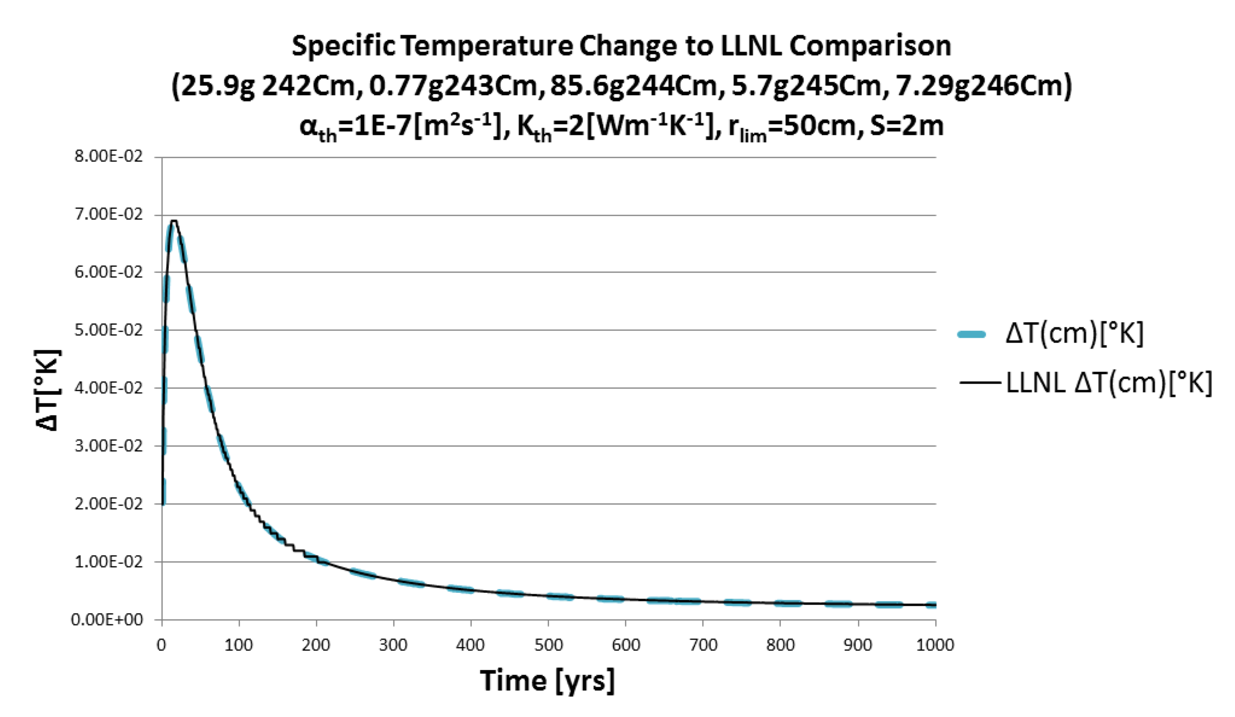
\includegraphics[width=\columnwidth]{./chapters/methodology/thermal_models/CmValidation.eps}
\end{center}
\caption{This comparison of \gls{STC} calculated thermal response from $Cm$ 
inventory per MTHM in 51GWd burnup UOX PWR fuel compares favorably with results 
from the semi-analytic model from LLNL.} 
\label{fig:CmValidation}
\end{figure}

\begin{figure}[htp!]
\begin{center}
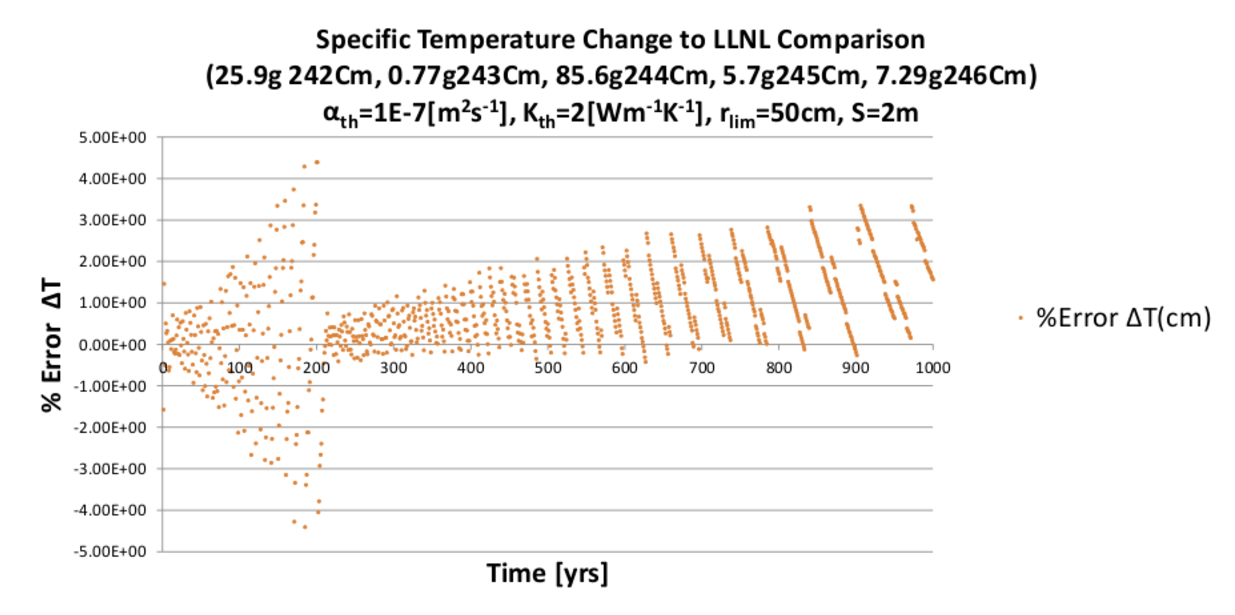
\includegraphics[width=\columnwidth]{./chapters/methodology/thermal_models/CmPercentError.eps}
\end{center}
\caption{Percent error between the semi-analytic model from LLNL and the \gls{STC} 
calculated thermal response from $Cm$ inventory per MTHM in 51GWd burnup UOX 
PWR fuel demonstrates a maximum percent error of 4.4\%.}
\label{fig:CmPercentError}
\end{figure}
% Unit Test Results
In addition to this validation effort, continual verification of code behavior 
is enabled by a suite of unit tests packaged with the tool. These tests are 
provided along with the source code so that they may be performed to evaluate 
the implementated behavior of units of functionality within the interpolation 
and specific temperature change algorithms even as the code is improved in the 
future.  

\subsection{Radionuclide Transport Toy Cases}

\begin{figure}[ht]
\centering
\includegraphics[width=0.6\textwidth]{./chapters/demonstration/base/drI.eps}
\caption[$^{235}U$ residence. Degradation Rate Waste Form No Release.]{
For Case DRI, in which total containment in the waste form is assumed ($F_{d,wf}=0$), 
$^{235}U$ takes up permanent residence in the waste form component.
}
\label{fig:drIall}
\begin{minipage}[b]{0.45\linewidth}

  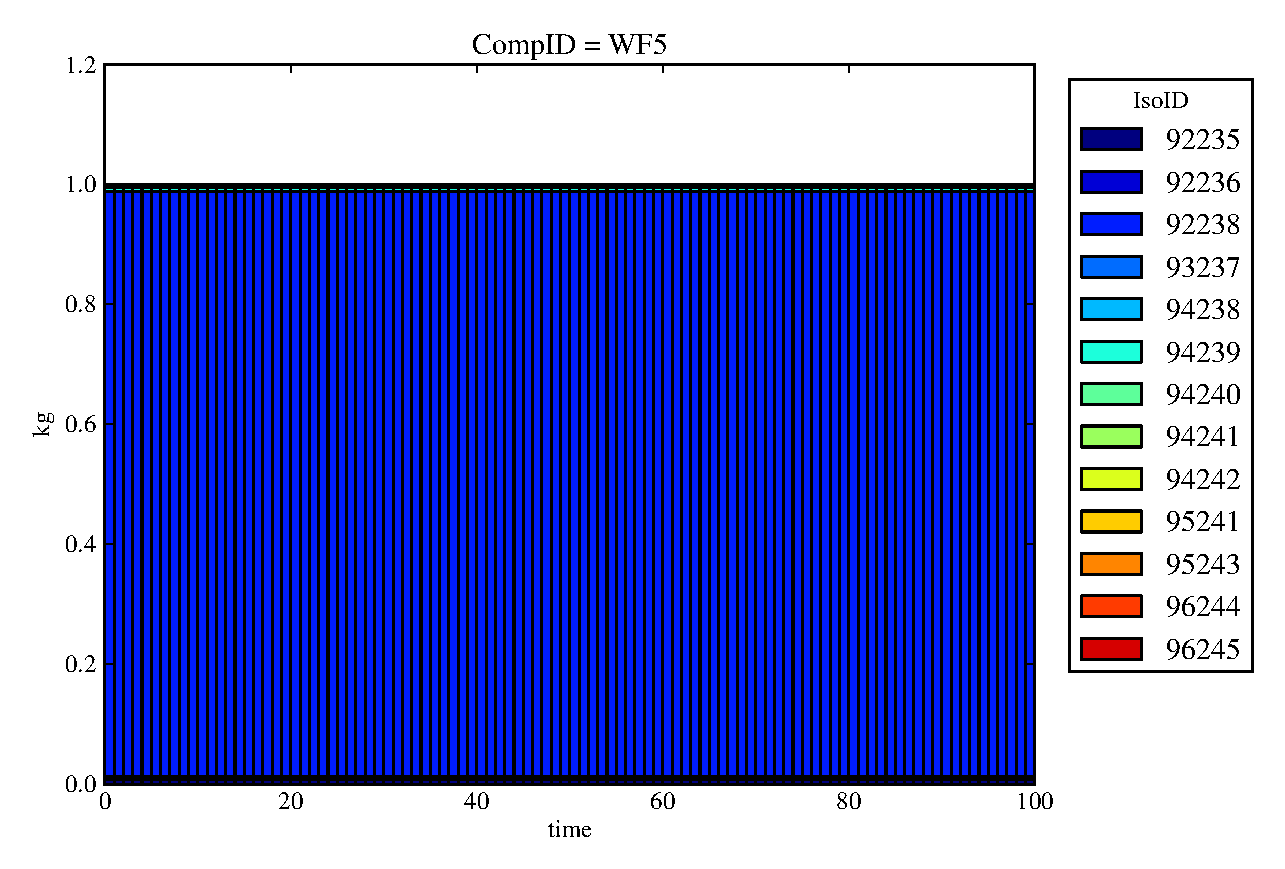
\includegraphics[width=\textwidth]{./chapters/demonstration/base/drI1.eps}
  \caption[DRI Waste Form Contaminants.]{
    Waste Form 5 ($F_d = 0$) never releases material.
    }
  \label{fig:drIwf5}
  
  \includegraphics[width=\textwidth]{./chapters/demonstration/base/drI3.eps}
  \caption[Case DRI Buffer Contaminants]{
    The Buffer, component 7 ($F_d = 0.1$), never recieves material.
    }
  \label{fig:drIbuff}

\end{minipage}
\hspace{0.05\linewidth}
\begin{minipage}[b]{0.45\linewidth}
  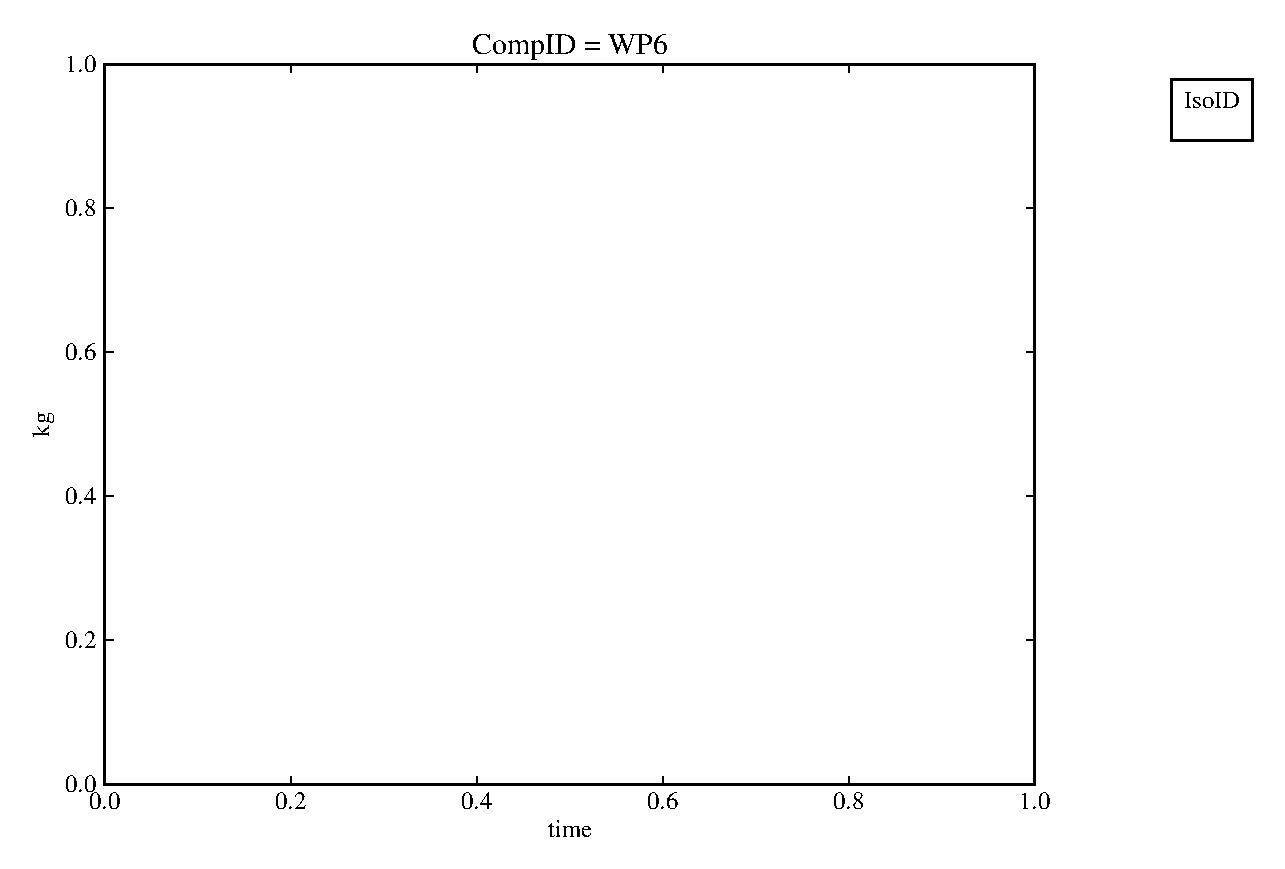
\includegraphics[width=\textwidth]{./chapters/demonstration/base/drI2.eps}
  \caption[Case DRI Waste Package Contaminants.]{ 
    Waste Package 6 ($F_d = 0.1$), never recieves material.
    }
  \label{fig:drIwp6}

  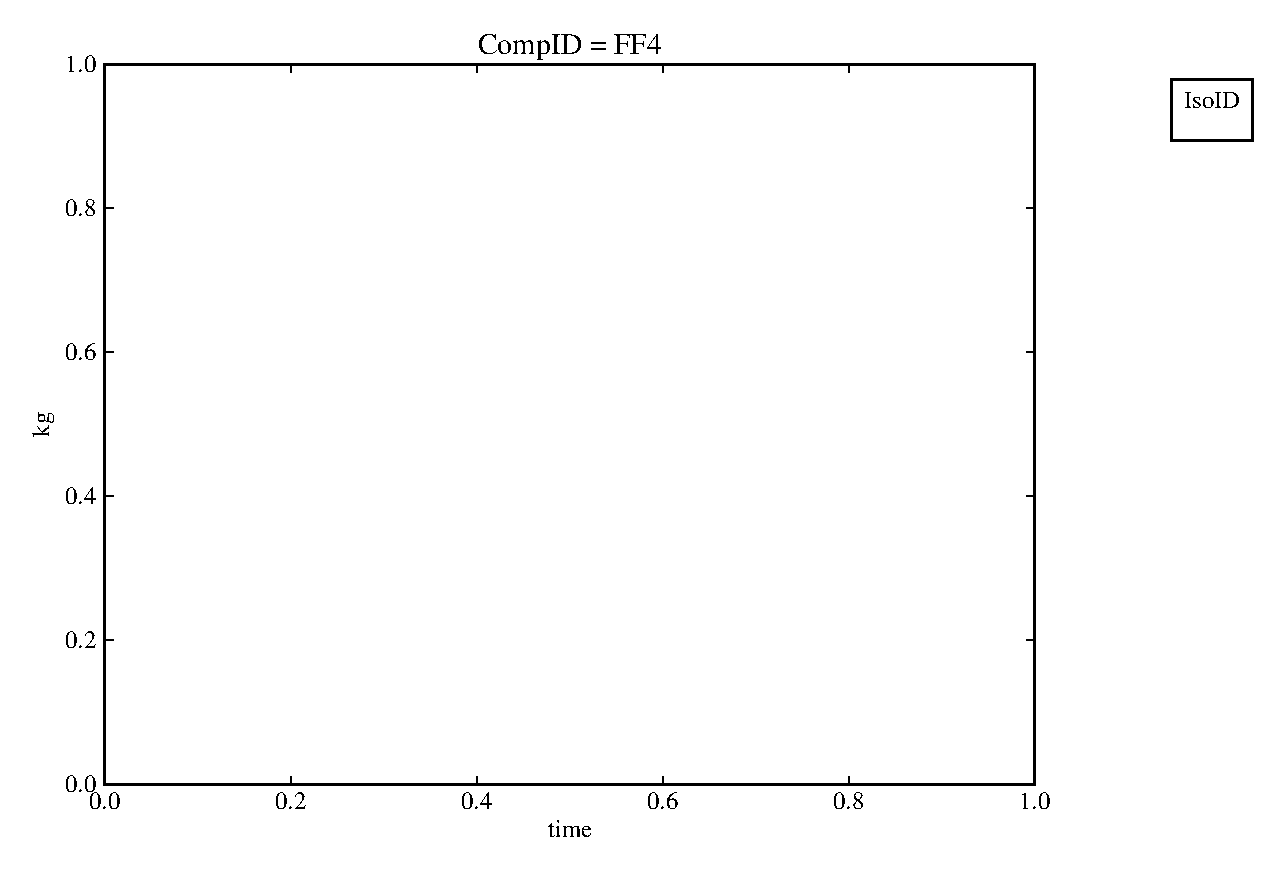
\includegraphics[width=\textwidth]{./chapters/demonstration/base/drI0.eps}
  \caption[Case DRI Far Field Contaminants.]{ 
    The Far Field, component 0 ($F_d = 0.1$), never recieves material.
    }
  \label{fig:drIff0}

  \end{minipage}
\end{figure}
\FloatBarrier



\begin{figure}[ht]
\centering
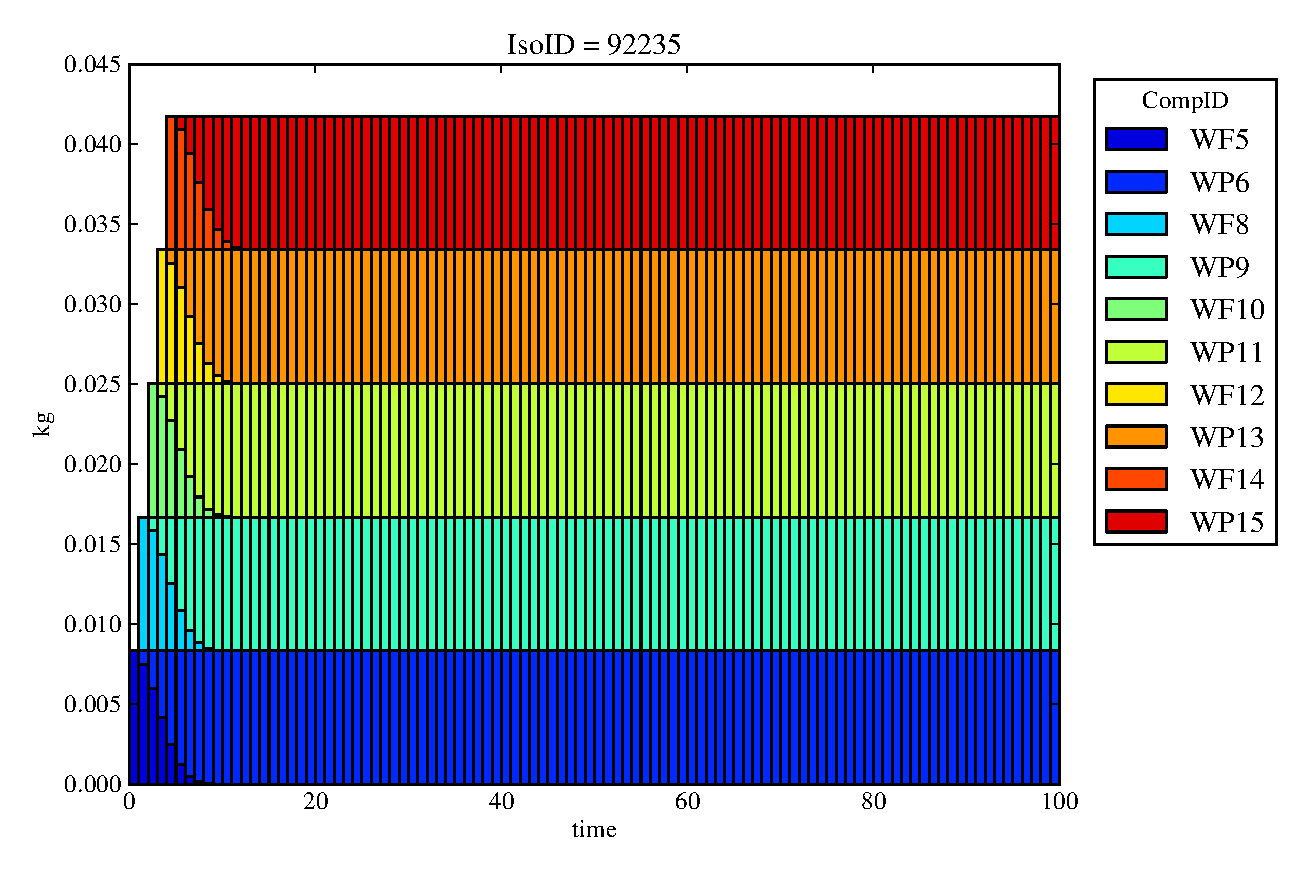
\includegraphics[width=0.6\textwidth]{./chapters/demonstration/base/drII.eps}
\caption[$^{235}U$ residence. Degradation Rate Waste Package No Release.]{
For Case DRII, in which total containment in the waste package is assumed ($F_{d,wp}=0$), 
$^{235}U$ travels through waste forms ($F_d = 0.1$) before 
permanent residence in the waste package components.
}
\label{fig:drIIall}
\begin{minipage}[b]{0.45\linewidth}

  \includegraphics[width=\textwidth]{./chapters/demonstration/base/drII1.eps}
  \caption[DRII Waste Form Contaminants.]{
    Waste Form 5 ($F_d = 0.1$) releases material with degradation. 
    }
  \label{fig:drIIwf5}
  
  \includegraphics[width=\textwidth]{./chapters/demonstration/base/drII3.eps}
  \caption[Case DRII Buffer Contaminants]{
    The Buffer, component 7 ($F_d = 0.1$), never recieves material.
    }
  \label{fig:drIIbuff}

\end{minipage}
\hspace{0.05\linewidth}
\begin{minipage}[b]{0.45\linewidth}
  \includegraphics[width=\textwidth]{./chapters/demonstration/base/drII2.eps}
  \caption[Case DRII Waste Package Contaminants.]{ 
    Waste Package 6 ($F_d = 0$) acheives total containment.
    }
  \label{fig:drIIwp6}

  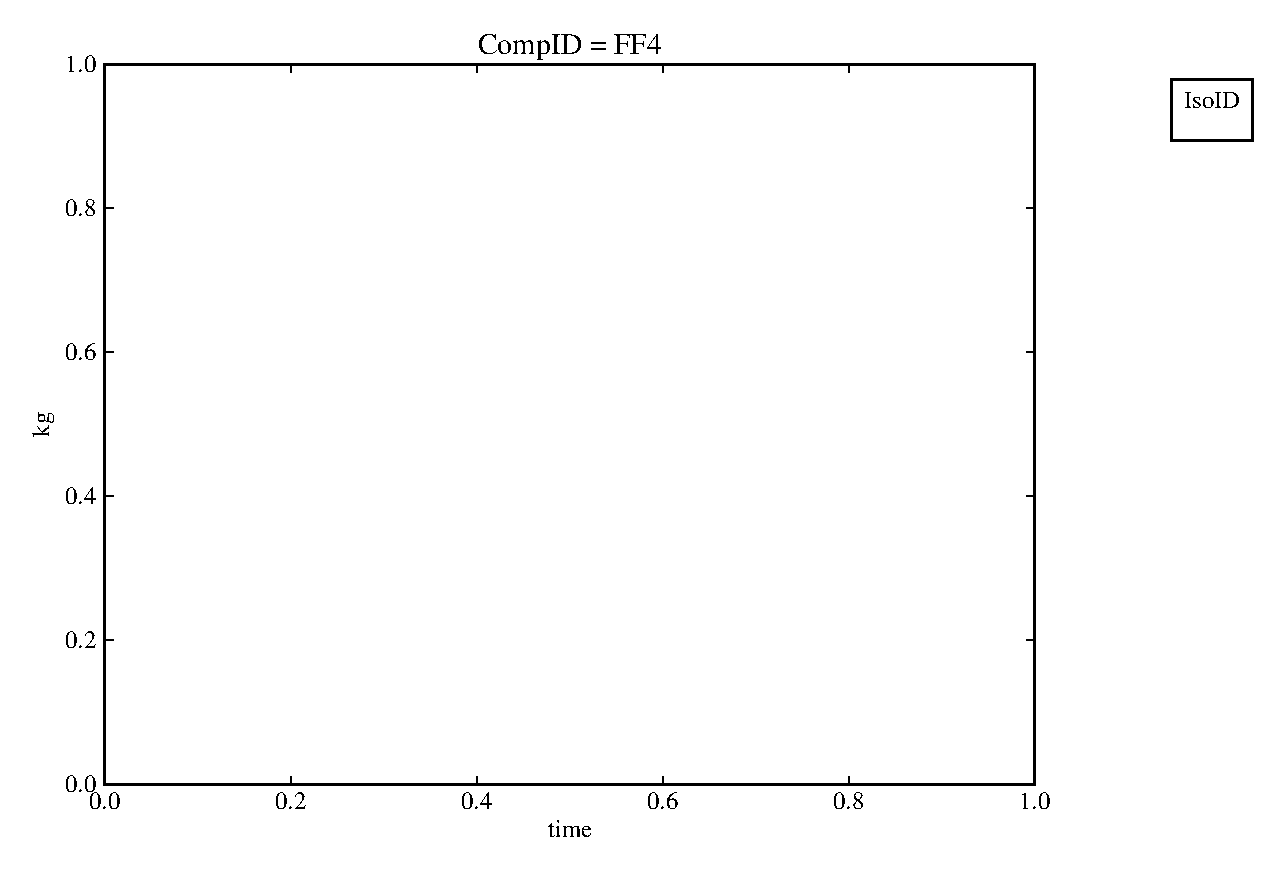
\includegraphics[width=\textwidth]{./chapters/demonstration/base/drII0.eps}
  \caption[Case DRII Far Field Contaminants.]{ 
    The Far Field, component 0 ($F_d = 0.1$), never recieves material.
    }
  \label{fig:drIIff0}


  \end{minipage}
\end{figure}
\FloatBarrier

\begin{figure}[ht]
\centering
\includegraphics[width=0.6\textwidth]{./chapters/demonstration/base/drIII.eps}
\caption[$^{235}U$ residence. Degradation Rate Buffer No Release.]{
For Case DRIII, in which total containment in the buffer is assumed ($F_{d,buffer}=0$), 
$^{235}U$ travels through waste forms and waste package components ($F_d = 0.1$) before 
permanent residence in the buffer component.
}
\label{fig:drIIIall}
\begin{minipage}[b]{0.45\linewidth}

  \includegraphics[width=\textwidth]{./chapters/demonstration/base/drIII1.eps}
  \caption[DRIII Waste Form Contaminants.]{
    Waste Form 5 ($F_d = 0.1$) releases material with degradation. 
    }
  \label{fig:drIIIwf5}
  
  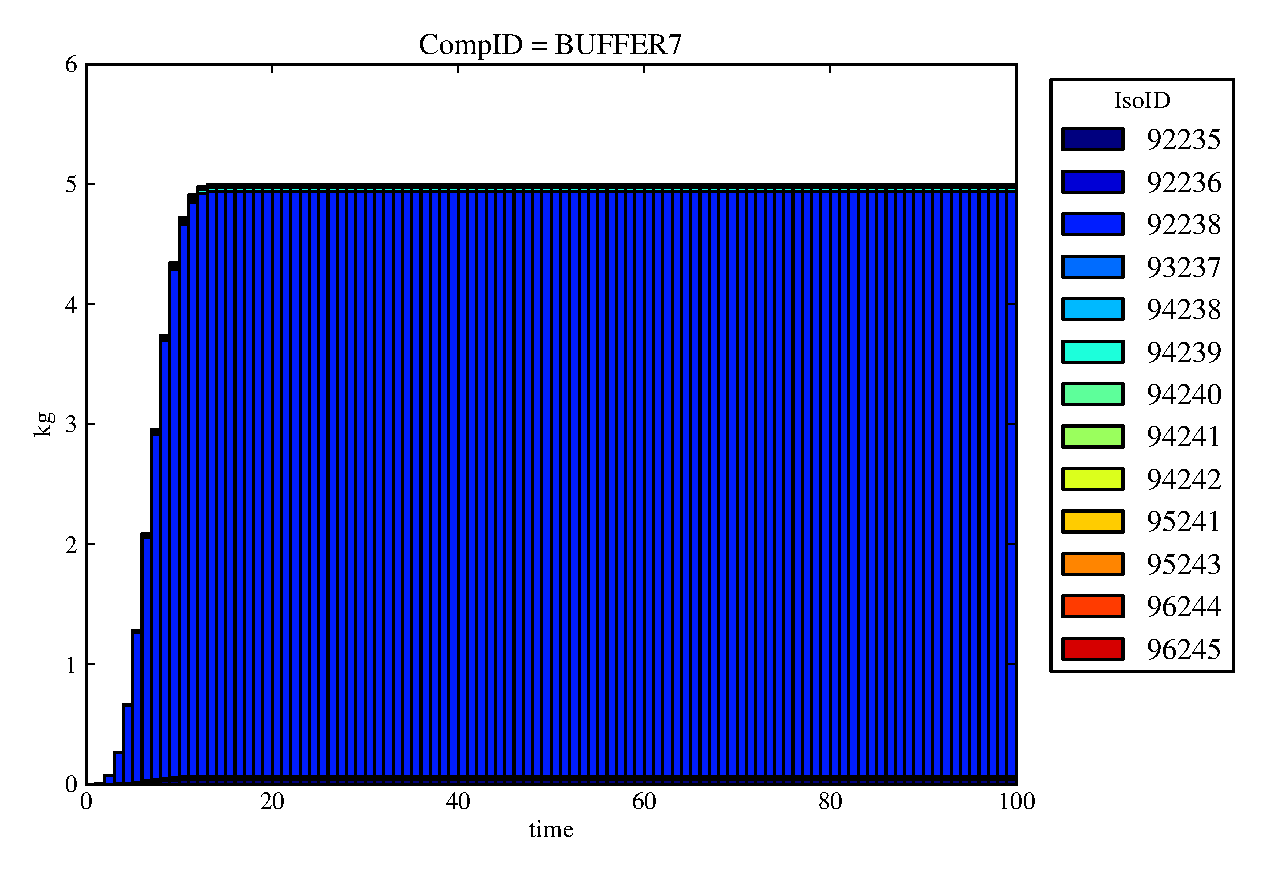
\includegraphics[width=\textwidth]{./chapters/demonstration/base/drIII3.eps}
  \caption[Case DRIII Buffer Contaminants]{
    The Buffer, component 7 ($F_d=0$), acheives total containment.
    }
  \label{fig:drIIIbuff}

\end{minipage}
\hspace{0.05\linewidth}
\begin{minipage}[b]{0.45\linewidth}
  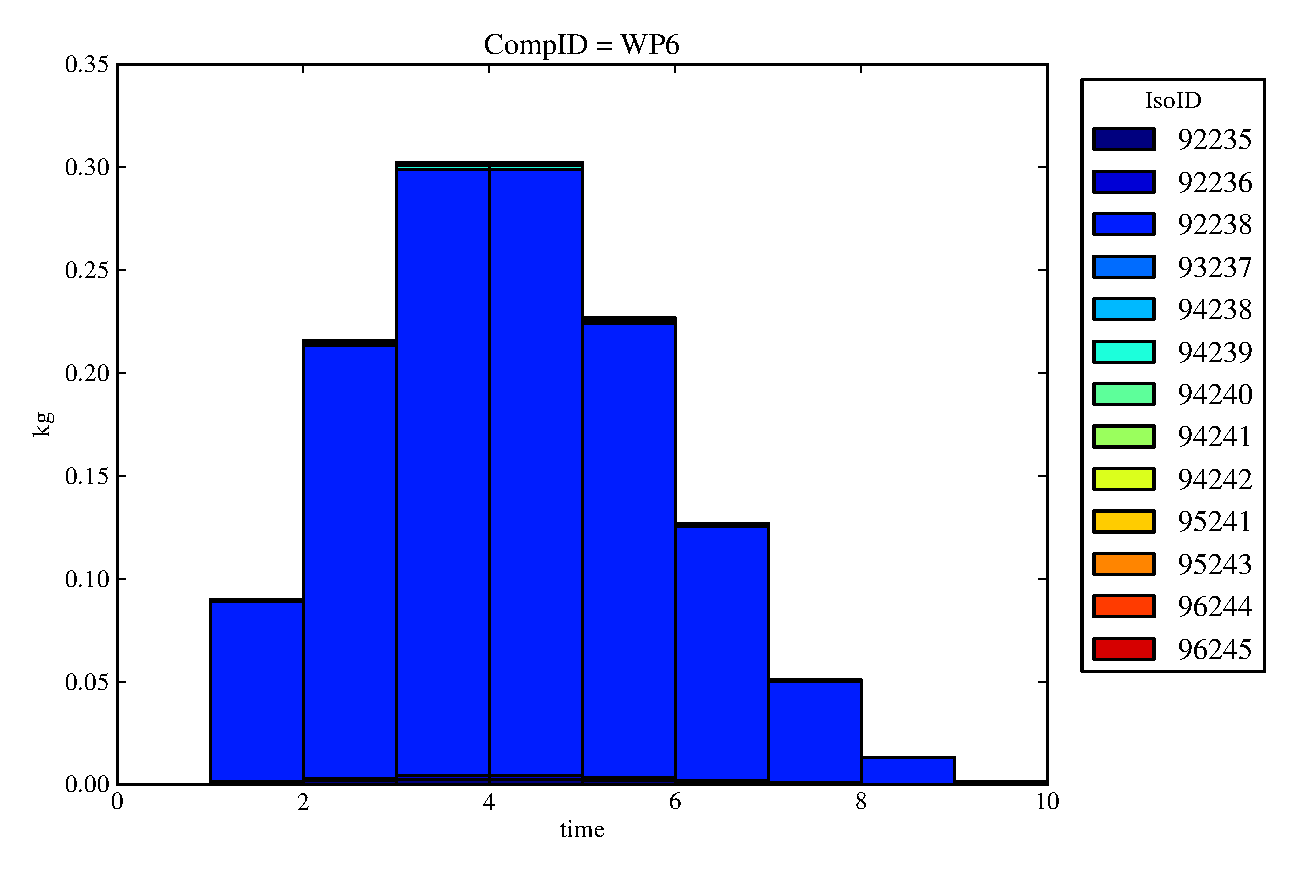
\includegraphics[width=\textwidth]{./chapters/demonstration/base/drIII2.eps}
  \caption[Case DRIII Waste Package Contaminants.]{ 
    Waste Package 6 ($F_d = 0.1$) recieves then releases material. 
    }
  \label{fig:drIIIwp6}

  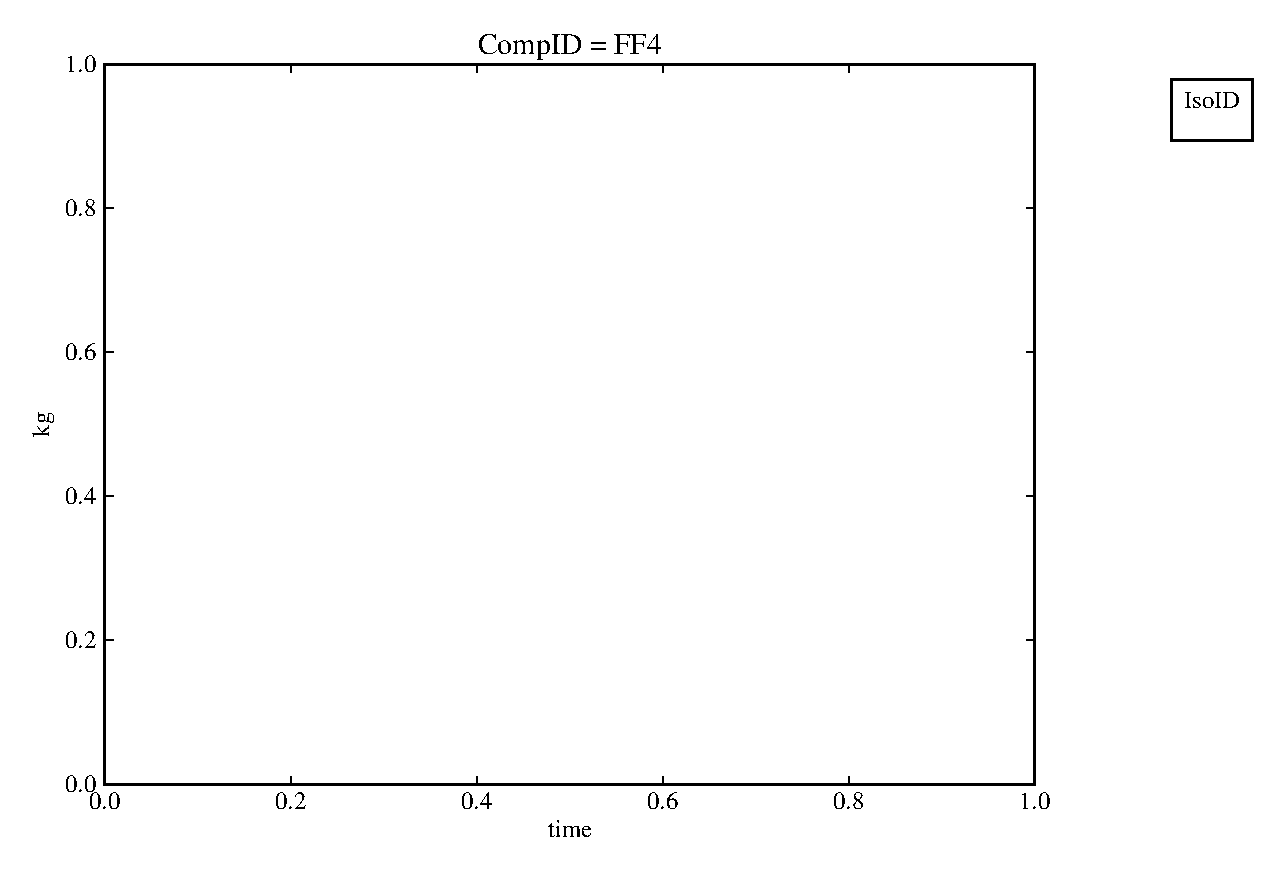
\includegraphics[width=\textwidth]{./chapters/demonstration/base/drIII0.eps}
  \caption[Case DRIII Waste Package Contaminants.]{ 
    The Far Field, component 0 ($F_d = 0.1$), never recieves material.
    }
  \label{fig:drIIIff0}


  \end{minipage}
\end{figure}
\FloatBarrier



\begin{figure}[ht]
\centering
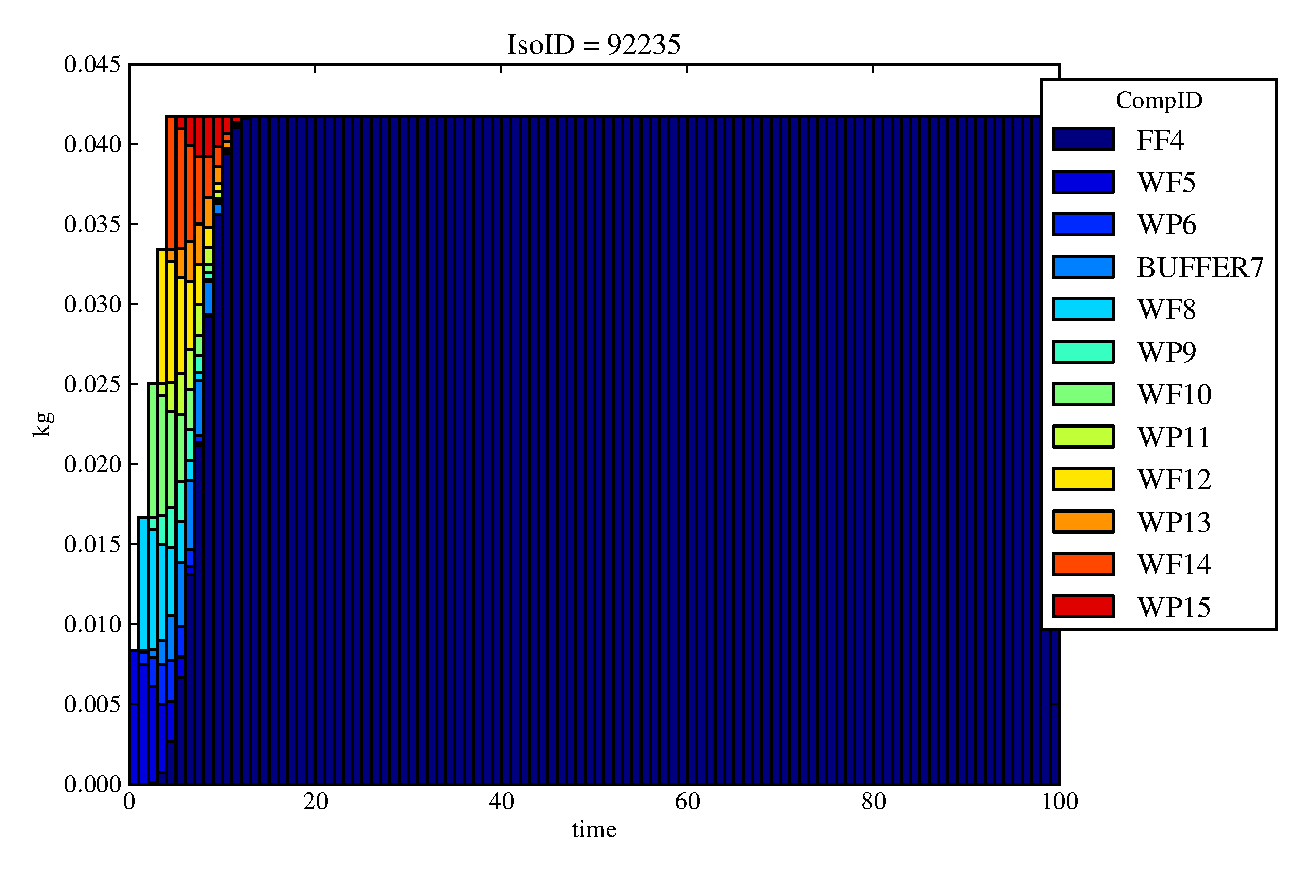
\includegraphics[width=0.6\textwidth]{./chapters/demonstration/base/drIV.eps}
\caption[$^{235}U$ residence. Degradation Rate Buffer No Release.]{
For DRIV case in which total containment in the far field is assumed ($F_{d,ff}=0$), 
$^{235}U$ travels through interior components ($F_d = 0.1$) before 
permanent residence in the far field component.
}
\label{fig:drIVall}
\begin{minipage}[b]{0.45\linewidth}

  \includegraphics[width=\textwidth]{./chapters/demonstration/base/drIV1.eps}
  \caption[DRIII Waste Form Contaminants.]{
    Waste Form 5 ($F_d = 0.1$) releases material with degradation. 
    }
  \label{fig:drIVwf5}
  
  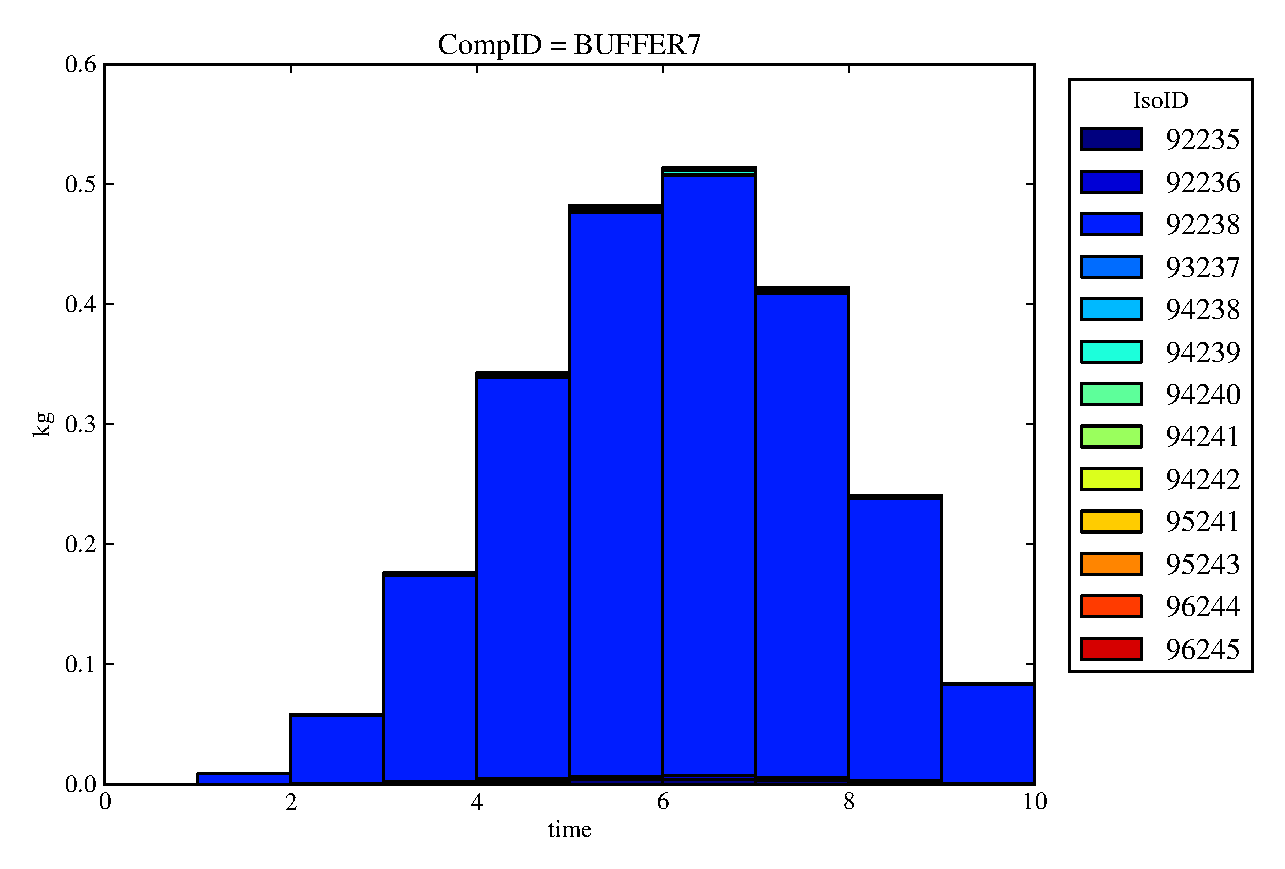
\includegraphics[width=\textwidth]{./chapters/demonstration/base/drIV3.eps}
  \caption[Case DRIII Buffer Contaminants]{
    The Buffer, component 7 ($F_d=0.0$), receives and then releases material.
    }
  \label{fig:drIVbuff}

\end{minipage}
\hspace{0.05\linewidth}
\begin{minipage}[b]{0.45\linewidth}
  \includegraphics[width=\textwidth]{./chapters/demonstration/base/drIV2.eps}
  \caption[Case DRIII Waste Package Contaminants.]{ 
    Waste Package 6 ($F_d = 0.1$) recieves then releases material. 
    }
  \label{fig:drIVwp6}

  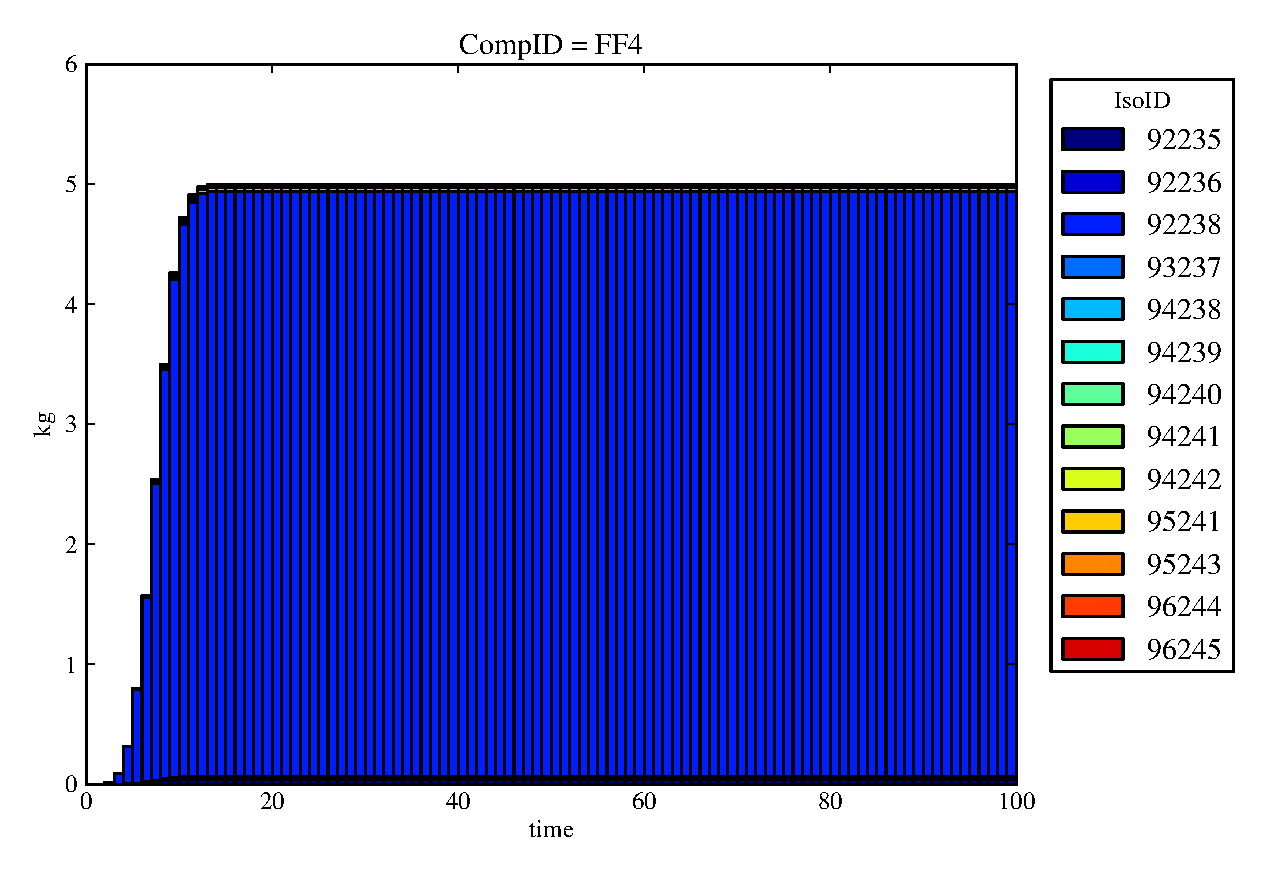
\includegraphics[width=\textwidth]{./chapters/demonstration/base/drIV0.eps}
  \caption[Case DRIII Waste Package Contaminants.]{ 
    The Far Field, component 0 ($F_d = 0.0$), acheives total containment.
    }
  \label{fig:drIVff0}


  \end{minipage}
\end{figure}


\begin{frame}[ctb!]
  \frametitle{Mixed Cell Model Base Case I}
\begin{figure}[ht]
\centering
\includegraphics[width=0.8\textwidth]{./images/mcI.eps}
\caption[$^{235}U$ residence. Mixed Cell Sorption Limitation Without Solubility Limitation.]{
For the MCI case in which total containment is only is assumed in the far field, 
but sorption and solubility limitation neglected, demonstrates results exactly similar to 
DRIV, as expected.}
\label{fig:mcI}
\end{figure}
\end{frame}

\begin{frame}[ctb!]
  \frametitle{Mixed Cell Model Base Case I}
  \begin{figure}[htbp!]
\begin{minipage}[b]{0.45\linewidth}

  \includegraphics[width=\textwidth]{./images/mcI1.eps}
  \caption[MCI Waste Form Contaminants.]{
    Waste Form 5 ($F_d = 0.1$) releases material with degradation. 
    }
  \label{fig:mcIwf5}
  
  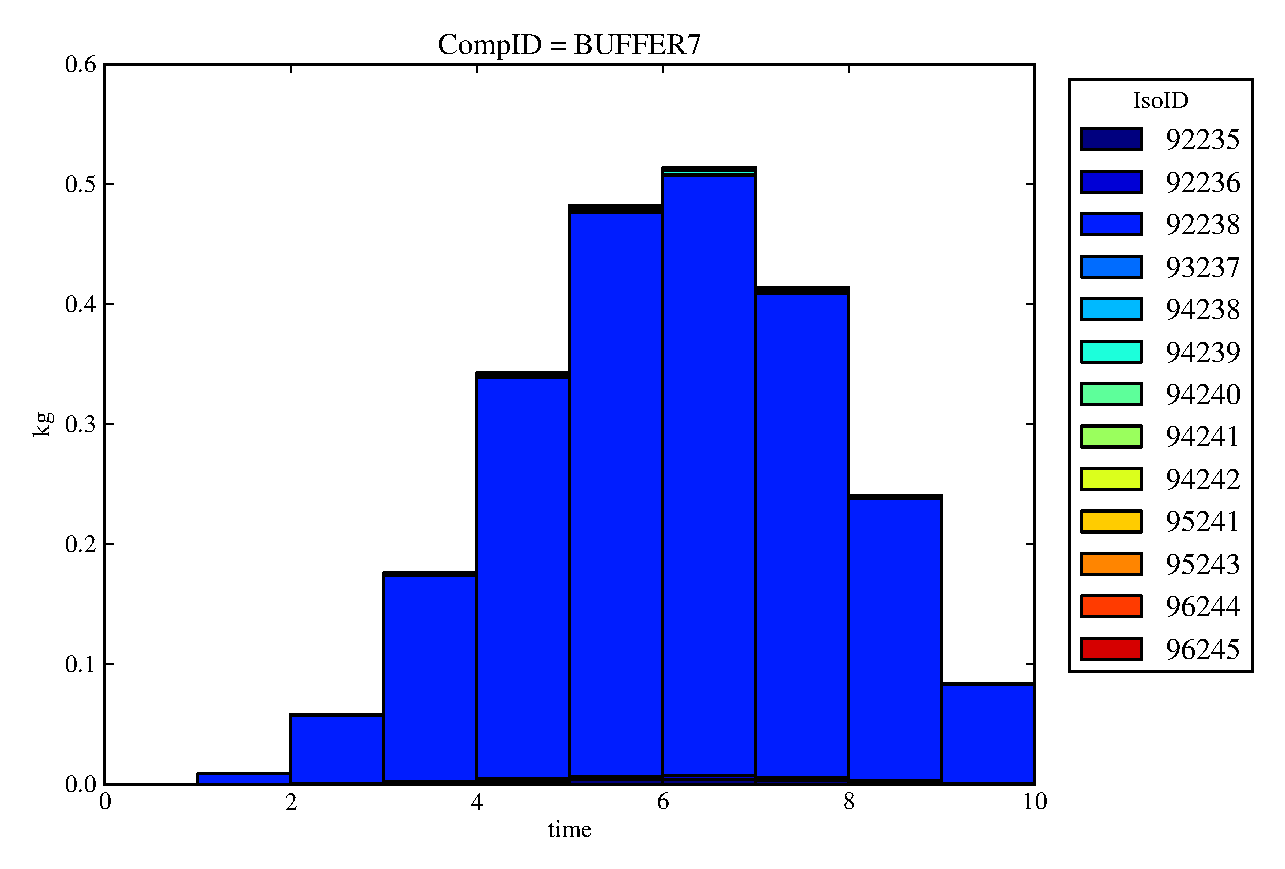
\includegraphics[width=\textwidth]{./images/mcI3.eps}
  \caption[Case MCI Buffer Contaminants]{
    The Buffer, component 7 ($F_d=0.1$), receives then releases material.
    }
  \label{fig:mcIbuff}

\end{minipage}
\hspace{0.05\linewidth}
\begin{minipage}[b]{0.45\linewidth}
  \includegraphics[width=\textwidth]{./images/mcI2.eps}
  \caption[Case MCI Waste Package Contaminants.]{ 
    Waste Package 6 ($F_d = 0.1$) recieves then releases material.
    }
  \label{fig:mcIwp6}

  \includegraphics[width=\textwidth]{./images/mcI0.eps}
  \caption[Case MCI Waste Package Contaminants.]{ 
    The Far Field, component 4 ($F_d = 0.0$), acheives full containment.
    }
  \label{fig:mcIff0}


  \end{minipage}
\end{figure}
\end{frame}

\begin{frame}[ctb!]
  \frametitle{Mixed Cell Model Base Case II}
\begin{figure}[ht]
\centering
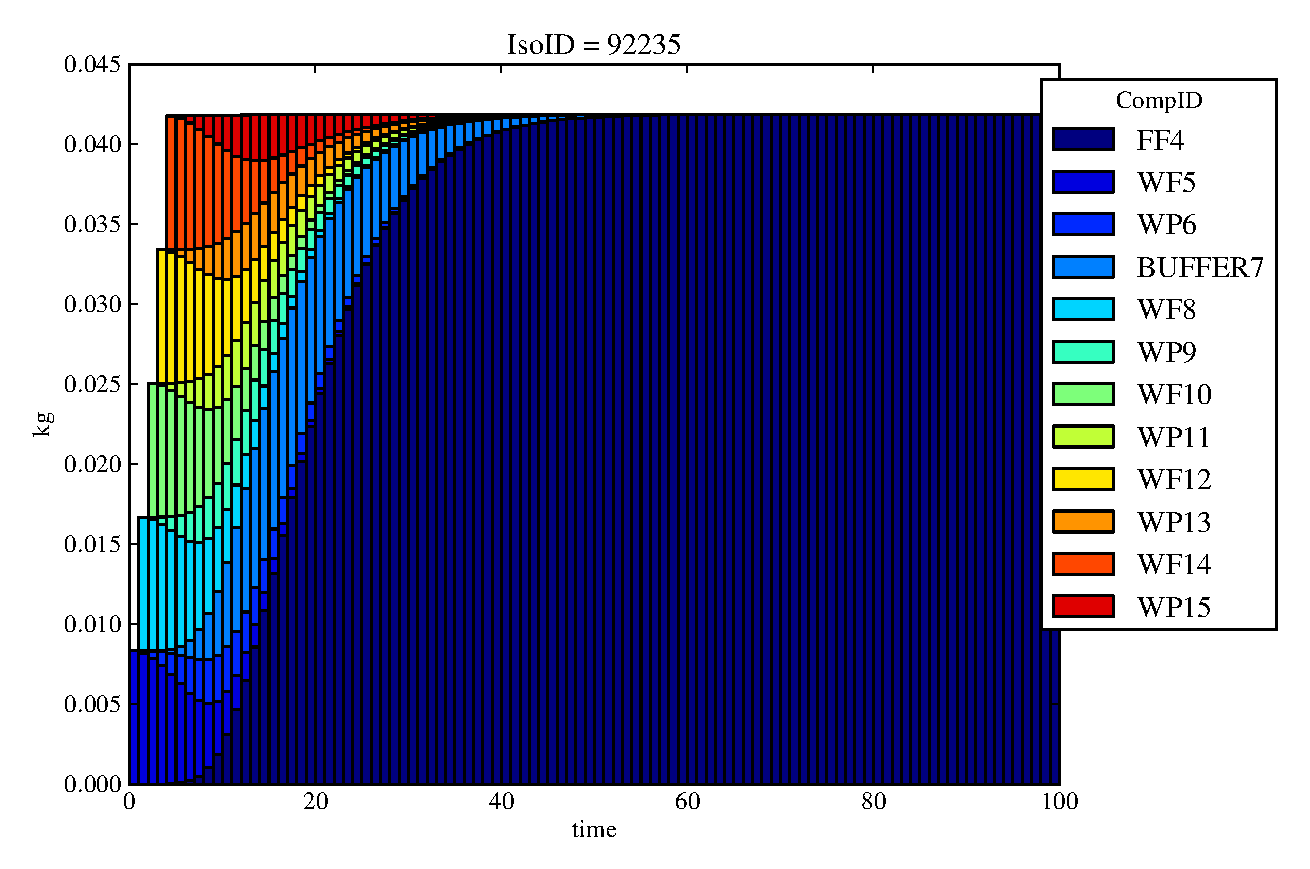
\includegraphics[width=0.8\textwidth]{./images/mcIII.eps}
\caption[$^{235}U$ residence. Mixed Cell Coupled Sorption and Solubility Limitation.]{
For the MCII case in which containment is affected by both sorption and 
solubility limitation,
($F_{d}=0.1$ for all components), $^{235}U$ travels more slowly than in the MCI case 
before permanent residence in the far field component.
}
\label{fig:mcIIIall}
\end{figure}
\end{frame}

\begin{frame}[ctb!]
  \frametitle{Mixed Cell Model Base Case II}
  \begin{figure}
\begin{minipage}[b]{0.45\linewidth}

  \includegraphics[width=\textwidth]{./images/mcIII1.eps}
  \caption[MCI Waste Form Contaminants.]{
    Waste Form 5 ($F_d = 0.1$) releases material with degradation. 
    }
  \label{fig:mcIIIwf5}
  
  \includegraphics[width=\textwidth]{./images/mcIII3.eps}
  \caption[Case MCI Buffer Contaminants]{
    The Buffer, component 7 ($F_d=0.1$), receives and then releases material.
    }
  \label{fig:mcIIIbuff}

\end{minipage}
\hspace{0.05\linewidth}
\begin{minipage}[b]{0.45\linewidth}
  \includegraphics[width=\textwidth]{./images/mcIII2.eps}
  \caption[Case MCI Waste Package Contaminants.]{ 
    Waste Package 6 ($F_d = 0.1$) recieves then releases material. 
    }
  \label{fig:mcIIIwp6}

  \includegraphics[width=\textwidth]{./images/mcIII0.eps}
  \caption[Case MCI Waste Package Contaminants.]{ 
    The Far Field, component 0 ($F_d = 0.1$), acheives total containment.
    }
  \label{fig:mcII}


  \end{minipage}
\end{figure}

\end{frame}


\begin{frame}[ctb!]
  \frametitle{Dispersion Model} 
\begin{figure}[ht]
\centering
\includegraphics[width=0.8\textwidth]{./images/lpDM_t_t.eps}
\caption[Lumped Parameter Dispersion Model Transit Time Sensitivity]{The transit time 
parameterization of the lumped parameter dispersion model of radionuclide 
transport has a strong effect on the material reaching the far field after 30 
years.  }
\label{fig:lp_t_t_begin}
\end{figure}
\end{frame}


\begin{frame}[ctb!]
\frametitle{Exponential Model} 
\begin{figure}[ht]
\centering
\includegraphics[width=0.8\textwidth]{./images/lpEXPM_t_t.eps}
\caption[Lumped Parameter Exponential Model Transit Time Sensitivity]{The transit time 
parameterization of the lumped parameter exponential model of radionuclide 
transport has a strong effect on the material reaching the far field after 30 
years.  }
\end{figure}
\end{frame}

\begin{frame}[ctb!]
\frametitle{Piston Flow Model} 
\begin{figure}[ht]
\centering
\includegraphics[width=0.8\textwidth]{./images/lpPFM_t_t.eps}
\caption[Lumped Parameter Piston Flow Model Transit Time Sensitivity]{The transit time 
parameterization of the lumped parameter piston flow model of radionuclide 
transport has a strong effect on the material reaching the far field after 30 
years.  }
\label{fig:lp_t_t_end}
\end{figure}

\end{frame}


\begin{figure}[ht]
\centering
\includegraphics[width=0.6\textwidth]{./chapters/demonstration/base/od.eps}
\caption[One Dimensional PPM Model.]{
For the case in which transport through all components is represented by the 1 
Dimensional PPM model, material moves very slowly into the far field. 
}
\label{fig:odall}
\begin{minipage}[b]{0.45\linewidth}

  \includegraphics[width=\textwidth]{./chapters/demonstration/base/od2.eps}
  \caption[Case ODI Waste Form Contaminants.]{
    Waste Form 5 slowly releases material into Waste Package 6.
    }
  \label{fig:drIVwf5}
  \includegraphics[width=\textwidth]{./chapters/demonstration/base/od3.eps}
  \caption[Case ODI Buffer Contaminants]{
    The Buffer, component 7 very slowly receives then releases material.
    }
  \label{fig:drIVbuff}
\end{minipage}
\hspace{0.05\linewidth}
\begin{minipage}[b]{0.45\linewidth}
  \includegraphics[width=\textwidth]{./chapters/demonstration/base/od1.eps}
  \caption[Case ODI Waste Package Contaminants.]{ 
    Waste Package 6 very slowly receives then releases material. 
    }
  \label{fig:drIVwp6}
  \includegraphics[width=\textwidth]{./chapters/demonstration/base/od0.eps}
  \caption[Case ODI Waste Package Contaminants.]{ 
    All material is released into Far Field, component 4.
    }
  \label{fig:drIVff0}


  \end{minipage}
\end{figure}


\subsection{Radionuclide Transport Validation Cases}
\begin{frame}[ctb!]
  \frametitle{Radionuclide Transport Validation Demonstrations}
\end{frame}

\subsection{Thermal Transport Toy Cases}

\begin{frame}[ctb!]
  \frametitle{Thermal Base Case Demonstration}
\begin{figure}[htp!]
\begin{center}
\includegraphics[width=\columnwidth]{./thermal_demonstration/CmValidation.eps}
\end{center}
\caption{This comparison of STC calculated thermal response from $Cm$ 
inventory per MTHM in 51GWd burnup UOX PWR fuel compares favorably with results 
from the semi-analytic model from LLNL.} 
\label{fig:CmValidation}
\end{figure}
\end{frame}


\begin{frame}[ctb!]
  \frametitle{Thermal Base Case Demonstration}
\begin{figure}[htp!]
\begin{center}
\includegraphics[width=\columnwidth]{./thermal_demonstration/CmPercentError.eps}
\end{center}
\caption{Percent error between the semi-analytic model from LLNL and the 
STC 
calculated thermal response from $Cm$ inventory per MTHM in 51GWd burnup UOX 
PWR fuel demonstrates a maximum percent error of 4.4\%.}
\label{fig:CmPercentError}
\end{figure}
\end{frame}


\subsection{Thermal Transport Validation Cases}
\begin{frame}[ctb!]
  \frametitle{Thermal Validation Demonstrations}
\end{frame}


\section{Conclusion}
\chapter{Conclusions}\label{ch:conclusion}
\section{Contributions}

This work has provided a repository anaylsis module for fuel cycle analysis 
that is the first of its kind. That is, it provides the first generic geology 
repository model integrated dynamically within a fuel cycle simulation code.

The Cyder source code in which these models are implemented as well as 
associated documentation are freely available to interested researchers and 
potential model developers. The application programming interface to this 
software library is intentionally general, facilitating the incorporation of 
the models presented here within external software tools in need of a 
multicomponent repository model.

Furthermore, this work contributes to an expanding ecosystem of computational 
models available for use with the Cyclus fuel cycle simulator. This hydrologic 
nuclide transport library, by virtue of its capability to modularly integrate 
with the Cyclus fuel cycle simulator has laid the foundation for integrated 
disposal option analysis in the context of fuel cycle options. 

\section{Suggested Future Work}

\begin{wbepi}{David C.~Makinson (1965)}
It is customary for authors of academic books to include in their prefaces statements such as this: ``I am indebted to ... for their invaluable help; however, any errors which remain are my sole responsibility.'' Occasionally an author will go further. Rather than say that if there are any mistakes then he is responsible for them, he will say that there will inevitably be some mistakes and he is responsible for them....

Although the shouldering of all responsibility is usually a social ritual, the admission that errors exist is not --- it is often a sincere avowal of belief. But this appears to present a living and everyday example of a situation which philosophers have commonly dismissed as absurd; that it is sometimes rational to hold logically incompatible beliefs.
\end{wbepi}

Above is the famous ``preface paradox,'' which illustrates how to use the \texttt{wbepi} environment for epigraphs at the beginning of chapters.  You probably also want to thank the Academy.

%%--------------------------------%%
%%--------------------------------%%
\begin{frame}[allowframebreaks]
  \frametitle{References}
  \bibliographystyle{plain}
  {\footnotesize \bibliography{defense} }

\end{frame}

%%--------------------------------%%


\appendix
\newcounter{finalframe}
\setcounter{finalframe}{\value{framenumber}}


\subsubsection{Advection vs. Diffusion Sensitivity GDSM Results}

In the parametric sensitivity analysis discussed in section
\ref{sec:AdvVelDiffCoeff}, it was shown that for isotopes of interest, higher
advective velocity and higher diffusivity lead to higher peak annual doses. 
However, the relationship between diffusivity and advective
velocity adds depth to the notion of a boundary between diffusive and advective
regimes.

The highly soluble and non-sorbing elements, $I$ and $Cl$ 
were expected to exhibit behavior that is highly sensitive 
to advection in the system in the advective regime but less sensitive to 
advection in the diffusive regime.  

In Figures \ref{fig:VAdvVelI129}, \ref{fig:VAdvVelI129VAdvVel}, 
\ref{fig:VAdvVelCl36}, and \ref{fig:VAdvVelCl36VAdvVel} , $^{129}I$ and 
$^{36}Cl$ are more sensitive to vertical advective velocity for lower vertical 
advective velocities. This demonstrates that for vertical advective velocities 
$6.31\times10^{-6}$ m/yr and above, lower reference diffusivities are 
ineffective at attenuating the mean of the peak doses for soluble, non-sorbing 
elements. 

\begin{figure}[htp!]
\begin{minipage}[b]{0.45\linewidth}
\centering
\includegraphics[width=\linewidth]{./chapters/nuclide_sensitivity/clay/AdvVelAndDiffCoeffEBSFail/I-129.eps}
\caption{$^{129}I$ reference diffusivity sensitivity.}
\label{fig:VAdvVelI129}

\end{minipage}
\hspace{0.05\linewidth}
\begin{minipage}[b]{0.45\linewidth}

\includegraphics[width=\linewidth]{./chapters/nuclide_sensitivity/clay/AdvVelAndDiffCoeffEBSFail/I-129-VAdvVel.eps}
\caption{$^{129}I$ vertical advective velocity sensitivity.}
\label{fig:VAdvVelI129VAdvVel}

\end{minipage}
\end{figure}

\begin{figure}[htp!]
\begin{minipage}[b]{0.45\linewidth}

\includegraphics[width=\textwidth]{./chapters/nuclide_sensitivity/clay/AdvVelAndDiffCoeffEBSFail/Cl-36.eps}
\caption{$^{36}Cl$ reference diffusivity sensitivity.}
\label{fig:VAdvVelCl36}

\end{minipage}
\hspace{0.05\linewidth}
\begin{minipage}[b]{0.45\linewidth}

\includegraphics[width=\textwidth]{./chapters/nuclide_sensitivity/clay/AdvVelAndDiffCoeffEBSFail/Cl-36-VAdvVel.eps}
\caption{$^{36}Cl$ vertical advective velocity sensitivity.}
\label{fig:VAdvVelCl36VAdvVel}
\end{minipage}
\end{figure}

The solubility limited and sorbing elements, $Tc$ and $Np$, in Figures 
\ref{fig:VAdvVelTc99}, \ref{fig:VAdvVelTc99VAdvVel}, \ref{fig:VAdvVelNp237}, and 
\ref{fig:VAdvVelNp237VAdvVel} show a very weak influence on peak annual dose 
rate for low reference diffusivities, but show a direct proportionality between 
dose and reference diffusivity above a threshold. For $^{99}Tc$, for example, 
that threshold occurs at $1\times10^{-11}$ m$^2$/s. 


Dose contribution from $^{99}Tc$ has a proportional 
relationship with vertical advective velocity above a regime threshold at 
$6.31\times10^{-5}$ m/yr, above which the system exhibits sensitivity to 
advection. 

%There is an interesting feature in which $^{99}Tc$ 
%exhibits a decrease in peak annual dose for an increase in reference diffusivity 
%for the very high ($6.31\times10^{-4}$) vertcial advective velocity case. %WHY? 

\begin{figure}[htp!]
\begin{minipage}[b]{0.45\linewidth}
\includegraphics[width=\linewidth]{./chapters/nuclide_sensitivity/clay/AdvVelAndDiffCoeffEBSFail/Tc-99.eps}
\caption{$^{99}Tc$ reference diffusivity sensitivity.}
\label{fig:VAdvVelTc99}

\end{minipage}
\hspace{0.05\linewidth}
\begin{minipage}[b]{0.45\linewidth}

\includegraphics[width=\linewidth]{./chapters/nuclide_sensitivity/clay/AdvVelAndDiffCoeffEBSFail/Tc-99-VAdvVel.eps}
\caption{$^{99}Tc$ vertical advective velocity sensitivity.}
\label{fig:VAdvVelTc99VAdvVel}

\end{minipage}
\end{figure}

\begin{figure}[htp!]
\begin{minipage}[b]{0.45\linewidth}
\includegraphics[width=\linewidth]{./chapters/nuclide_sensitivity/clay/AdvVelAndDiffCoeffEBSFail/Np-237.eps}
\caption{$^{237}Np$ reference diffusivity sensitivity.}
\label{fig:VAdvVelNp237}

\end{minipage}
\hspace{0.05\linewidth}
\begin{minipage}[b]{0.45\linewidth}

\includegraphics[width=\linewidth]{./chapters/nuclide_sensitivity/clay/AdvVelAndDiffCoeffEBSFail/Np-237-VAdvVel.eps}
\caption{$^{237}Np$ vertical advective velocity sensitivity.}
\label{fig:VAdvVelNp237VAdvVel}
  
\end{minipage}
\end{figure}

The convergence of the effect of the reference diffusivity and vertical 
advective velocity for the cases above shows the effect of dissolved 
concentration (solubility) limits and sorption. $Se$ is non-sorbing, but 
solubility limited.  The results from $^{79}Se$ in Figure \ref{fig:VAdvVelSe79} 
and \ref{fig:VAdvVelSe79VAdvVel} show that for low vertical advective velocity, 
the system is diffusion dominated.  However, for high vertical advective 
velocity, the diffusivity remains important even in the advective regime as 
spreading facilitates transport in the presence of solubility limited transport. 

\begin{figure}[htp!]
\begin{minipage}[b]{0.45\linewidth}
\centering
\includegraphics[width=\linewidth]{./chapters/nuclide_sensitivity/clay/AdvVelAndDiffCoeffEBSFail/Se-79.eps}
\caption{$^{79}Se$ reference diffusivity sensitivity.}
\label{fig:VAdvVelSe79}

\end{minipage}
\hspace{0.05\linewidth}
\begin{minipage}[b]{0.45\linewidth}

\includegraphics[width=\linewidth]{./chapters/nuclide_sensitivity/clay/AdvVelAndDiffCoeffEBSFail/Se-79-VAdvVel.eps}
\caption{$^{79}Se$ vertical advective velocity sensitivity.}
\label{fig:VAdvVelSe79VAdvVel}

\end{minipage}
\end{figure}
\FloatBarrier

\begin{frame}[ctb!]
\frametitle{Cyder Advective Diffusive Sensitivity}
\begin{figure}[ht]
\centering
\includegraphics[height=0.7\textheight]{./nuclide_demonstration/adv_vel_diff.eps}
\caption[Advection vs. Diffusion Sensitivity in Cyder]{Dual advective velocity 
and reference diffusivity sensitivity for a non-sorbing, infinitely soluble 
nuclide. This demonstration utilized the Degradation Rate model and the coupled 
advective dispersive mass transfer mode.}
\label{fig:dr_adv_diff}
\end{figure}
\end{frame}


\section{LLNL Model Background}
% LLNL
\subsection{Analytical Model Background}
\begin{frame}[ctb!]
\frametitle{Analytical Model : Background}
The analytical  model
\begin{itemize} 
  \item was created at LLNL (H. Greenberg, J. Blink, et. al) \cite{hardin_generic_2011, sutton_investigations_2011, 
greenberg_application_2012}
  \item employs an analytic model from Carslaw and Jaeger \cite{carslaw_conduction_1959} 
  \item is implemented in MathCAD \cite{ptc_mathcad_2010}
  \item seeks to inform heat limited waste capacity calculations for 
    \begin{itemize}
      \item arbitrary geology 
      \item arbitrary waste package loading densities
      \item arbitrary homogeneous decay heat source
    \end{itemize}
\end{itemize}
\end{frame}

\begin{frame}
  \frametitle{Analytical Model : Geometry}
  \begin{figure}[h!]
    \begin{center}
      \includegraphics[width=0.7\textwidth]{./images/llnlConcept.eps}
    \caption{Vertical, horizontal, alcove, and borehole emplacement layouts can 
    be represented by a line of point sources and adjacent line sources 
    \cite{sutton_investigations_2011}.}
    \label{fig:llnl}
    \end{center}
  \end{figure}
\end{frame}

\begin{frame}
  \frametitle{Analytical Model : Calculation Method}
    LLNL's model is a MathCAD solution of the transient homogeneous 
    conduction equation,
    \begin{align}
      \nabla^2T  = \frac{1}{\alpha}\frac{\partial T}{\partial t},
      \label{condGl}
    \end{align}
    in which superimposed point and line source solutions approximate the repository 
    layout.
\end{frame}

\begin{frame}[ctb!]
\frametitle{Analytical Model : Calculation Method}
The model consists of two conceptual regions, an external region representing 
the host rock and an internal region representing the waste form, package, and 
buffer Engineered Barrier System within the disposal tunnel wall.   
\begin{itemize}
  \item Since the thermal mass of the EBS is small in comparison to the thermal 
    mass of the host rock, the internal region may be treated as quasi-steady 
    state.
  \item The transient state of the temperature at the calculation radius is 
    found with a convolution of the transient external solution with the steady 
    state internal solution.
  \item The internal and external regions are \textbf{approximated} to be a 
    single homogeneous medium.
  \item The process is then iterated with a one year resolution in order to 
    arrive at a temperature evolution over the lifetime of the repository. 
\end{itemize}
\end{frame}


\begin{frame}[ctb!]
\frametitle{Analytical Model : Calculation Method}
\begin{minipage}{0.3\textwidth}
\begin{figure}[h!]
  \begin{center}
    \includegraphics[width=\textwidth]{./images/llnlConcept.eps}
  \end{center}
  \caption{The central package is represented by a finite line source
  \cite{sutton_investigations_2011}.}
  \label{fig:llnl}
\end{figure}
\end{minipage}
\hspace{0.01mm}
\begin{minipage}{0.6\textwidth}
The geometric layout of the analytic LLNL model in Figure \ref{fig:llnl} 
shows  that the central package is represented by the finite line solution
\footnotesize{
\begin{align}
  T_{line}&(t,x,y,z) = \nonumber\\
  &\frac{1}{8\pi K_{th}} 
  \bigintsss_0^t\!\frac{q_L(t')}{t-t'}e^{ \frac{-\left(x^2 + z^2\right)}{4\alpha 
  (t-t')} }\nonumber\\ &\cdot\left[ \erf{\left[ \frac{1}{2} \frac{\left( y + 
  \frac{L}{2} \right)}{\sqrt{\alpha(t-t')}}  \right]} - \erf{\left[ \frac{1}{2} 
  \frac{\left( y - \frac{L}{2} \right)}{\sqrt{\alpha(t-t')}}  \right]} 
  \right]\,\mathrm{dt'}.
  \label{line}
\end{align}
}
\end{minipage}
\end{frame}

\begin{frame}[ctb!]
\frametitle{Analytical Model : Calculation Method}
\begin{minipage}{0.3\textwidth}
\begin{figure}[h!]
  \begin{center}
    \includegraphics[width=\textwidth]{./images/llnlConcept.eps}
  \end{center}
  \caption{Adjacent packages are represented as point sources
  \cite{sutton_investigations_2011}.}
  \label{fig:llnl}
\end{figure}
\end{minipage}
\hspace{0.1mm}
\begin{minipage}{0.6\textwidth}
 Adjacent packages within the central tunnel are represented by the point source 
 solution,
 \footnotesize{
  \begin{align}
    T_{point}(t,r) &= \frac{1}{8K_{th}\sqrt{\alpha}\pi^{\frac{3}{2}}}\nonumber\\
     &\bigintsss_0^{t}\!\frac{q(t')}{(t-t')^{\frac{3}{2}}}e^{\frac{-r^2}{4\alpha(t-t')}}\,\mathrm{dt'}.
    \label{point}
  \end{align}
  }
  \end{minipage}
\end{frame}


\begin{frame}[ctb!]
\frametitle{Analytical Model : Calculation Method}
\begin{minipage}{0.3\textwidth}
\begin{figure}[h!]
  \begin{center}
    \includegraphics[width=\textwidth]{./images/llnlConcept.eps}
  \end{center}
  \caption{The non-central disposal tunnels are represented as infinite line sources
  \cite{sutton_investigations_2011}.}
  \label{fig:llnl}
\end{figure}
\end{minipage}
\hspace{0.1mm}
\begin{minipage}{0.6\textwidth}
Adjacent disposal tunnels are represented by the infinite line source solution,
\footnotesize{
\begin{align}
  T_{\infty line}(t,x,z) &= \frac{1}{4\pi K_{th}} 
  \bigintsss_0^t\frac{q_L(t')}{t-t'}e^{ \frac{-\left(x^2 + z^2\right)}{4\alpha 
  (t-t')} }
  \label{infline}
  \intertext{in infinite homogeneous media, where}
  \alpha &= ~~\mbox{thermal diffusivity } [m^2\cdot s^{-1}]\nonumber\\
  q(t) &= ~~\mbox{point heat source} [W]\nonumber\\
  \intertext{and}
  q_L(t) &= ~~\mbox{linear heat source} [W\cdot m^{-1}]\nonumber
\end{align}
}
Superimposed point and line source solutions allow for a notion of the 
repository layout to be modeled in the host rock.
\end{minipage}
\end{frame}



\section{Geologic Media and Concepts}
\begin{frame}[ctb!]
  \frametitle{Clay Disposal Environments}
  \footnotesize{

  \begin{figure}[h!]
    \begin{center}
      \includegraphics[height=.7\textheight]{./images/belgianClayRedImp.eps}
    \end{center}
    \caption{Belgian reference concept in Boom Clay 
    \cite{von_lensa_red-impact_2008}.}
    \label{fig:belgianClayRedImp}
  \end{figure}

}
\end{frame}

\begin{frame}[ctb!]
  \frametitle{Granite Disposal Environments}
  \footnotesize{

  \begin{figure}[h!]
    \begin{center}
      \includegraphics[height=.7\textheight]{./images/czechGraniteRedImp.eps}
    \end{center}
    \caption{Czech reference concept in Granite 
    \cite{von_lensa_red-impact_2008}.}
    \label{fig:czechGraniteRedImp}
  \end{figure}
}
\end{frame}

\begin{frame}[ctb!]
  \frametitle{Salt Disposal Environments}
  \footnotesize{

  \begin{figure}[h!]
    \begin{center}
      \includegraphics[height=.7\textheight]{./images/carter_salt_layout.eps}
    \end{center}
    \caption{DOE-NE Used Fuel Disposition Campaign  concept in 
    Salt \cite{hardin_generic_2011}.}
    \label{fig:salt_layout}
  \end{figure}
}
\end{frame}
\begin{frame}[ctb!]
  \frametitle{Salt Disposal Environments}
  \footnotesize{

  \begin{figure}[h!]
    \begin{center}
      \includegraphics[height=.7\textheight]{./images/hardin_salt_layout.eps}
    \end{center}
    \caption{DOE-NE Used Fuel Disposition Campaign  concept in 
    Salt \cite{hardin_generic_2011}.}
    \label{fig:hardin_salt_layout}
  \end{figure}
}
\end{frame}

\begin{frame}[ctb!]
  \frametitle{Deep Borehole Disposal Environment}
  \footnotesize{

  \begin{figure}[h!]
    \begin{center}
      \includegraphics[height=.7\textheight]{./images/boreholeGPAM.eps}
    \end{center}
    \caption{DOE-NE Used Fuel Disposition Campaign Deep Borehole concept 
    \cite{hardin_generic_2011}.}
    \label{fig:boreholeGPAM}
  \end{figure}
}
\end{frame}

%%----------------------------------------%%
\begin{frame}[ctb!]
  \frametitle{Engineered Barriers : Waste Forms}
\footnotesize{
  The first line of defense is the waste form.
  \begin{figure}[htbp!]
  \begin{center}
    \includegraphics[width=0.5\textwidth]{./images/waste_forms_poinssot.eps}
  \end{center}
  \caption{A comparison of uranium oxide and borosilicate glass waste forms 
  \cite{poinssot_long-term_2012}.}
  \label{fig:waste_forms_poinssot}
\end{figure}

}
\end{frame}

%%----------------------------------------%%
\begin{frame}[ctb!]
  \frametitle{Engineered Barriers : Waste Packages}
\footnotesize{
  \begin{figure}[htbp!]
  \begin{center}
    \includegraphics[width=0.7\textwidth]{./images/packages_ineel.eps}
  \end{center}
  \caption{Conceptual mockup of waste packages around waste forms 
    \cite{bridges_standardized_2001}.}
  \label{fig:packages}
\end{figure}

}
\end{frame}

%%----------------------------------------%%
\begin{frame}[ctb!]
  \frametitle{Engineered Barriers : Disposal Cask}
\footnotesize{
  \begin{figure}[htbp!]
  \begin{center}
    \includegraphics[width=0.7\textwidth]{./images/cask_ineel.eps}
  \end{center}
  \caption{Conceptual mockup of a transport and disposal cask 
    \cite{bridges_standardized_2001}.}
  \label{fig:packages}
\end{figure}

}
\end{frame}

%%----------------------------------------%%
\begin{frame}[ctb!]
  \frametitle{Engineered Barriers : Buffer}
\footnotesize{
  \begin{figure}[h!]
    \begin{center}
      \includegraphics[height=.7\textheight]{./images/belgianClayRedImp.eps}
    \end{center}
    \caption{Belgian reference concept in Boom Clay 
    \cite{von_lensa_red-impact_2008}.}
    \label{fig:belgianClayRedImp}
  \end{figure}
}
\end{frame}

%%----------------------------------------%%
\begin{frame}[ctb!]
  \frametitle{Natural Barrier : Geology}
\footnotesize{
  \begin{figure}[htbp!]
  \begin{center}
    \includegraphics[width=0.7\textwidth]{./images/wipp_stratigraph.eps}
  \end{center}
  \caption{The Waste Isolation Pilot Plant has many geologic layers above the 
    salt bed \cite{doe_wipp_2013}.}
  \label{fig:wipp}
\end{figure}

}
\end{frame}
\begin{frame}
  \frametitle{Repository Layouts}

  \begin{minipage}{0.49\textwidth}
    \begin{figure}[h!]
      \includegraphics[width=0.75\textwidth]{./images/boreholes.eps}
    \end{figure}
    \begin{figure}[h!]
      \includegraphics[width=0.75\textwidth]{./images/vertical.eps}
    \end{figure}
  \end{minipage}
  \hspace{0.01cm}
  \begin{minipage}{0.49\textwidth}
    \begin{figure}[h!]
      \includegraphics[width=0.8\textwidth]{./images/horizontal.eps}
    \end{figure}
    \begin{figure}[h!]
      \includegraphics[width=0.8\textwidth]{./images/alcoves.eps}
    \end{figure}
  \end{minipage}

\end{frame}

\begin{frame}[ctb!]
  \footnotesize{
  \frametitle{Unsaturated, Ventilated Concepts}
  \begin{figure}[htbp!]
  \begin{center}
    \includegraphics[height=0.7\textwidth]{./images/yucca_tunnel.eps}
  \end{center}
  \caption{The current U.S. geologic disposal concept \cite{peters_whats_2013}.}
  \label{fig:yucca_tunnel}
\end{figure}

}
\end{frame}

\begin{frame}[ctb!]
  \footnotesize{
  \frametitle{Saturated , Enclosed Concepts} 
 \begin{figure}[h!]
    \begin{center}
      \includegraphics[height=.7\textheight]{./images/belgianClayRedImp.eps}
    \end{center}
    \caption{The Belgian reference concept in Boom Clay is backfilled very soon
   after waste emplacement without a ventilation period and is located below the water table
   \cite{von_lensa_red-impact_2008}.}
    \label{fig:belgianClayRedImp}
  \end{figure}
}
\end{frame}

\setcounter{framenumber}{\value{finalframe}}
\section{Mixed Cell Model}

\begin{frame}
  \frametitle{Radionuclide Transport : Mixed Cell Sorption}
  \footnotesize{

The mass of contaminant sorbed into the degraded and precipitated solids can be
found using a linear isotherm model \cite{schwartz_fundamentals_2004},
characterized by the relationship 
\begin{align}
s_{i} &= K_{di} c_{i}
\label{linear_iso}
\intertext{where}
s_i &= \mbox{ the solid concentration of isotope i }[kg/kg]\nonumber\\
K_{di} &= \mbox{ the distribution coefficient of isotope i}[m^3/kg]\nonumber\\
c_i &= \mbox{ the liquid concentration of isotope i }[kg/m^3].\nonumber
\end{align}

  From the sorbed contaminant mass, we find the non-sorbed contaminant mass in the free fluid,

\begin{align}
m_{ffl}   &= m_{ffT} - \frac{1}{2} \left(m_{ffT} - m_{psm} - \frac{V_{ff}}{K_d}\right) \nonumber\\
          & \mp \frac{1}{2} \sqrt{m_{ffT}^2 + 2m_{ffT}\left(m_{psm} - 
          \frac{V_{ff}}{K_d}\right) + \left(m_{psm} + 
          \frac{V_{ff}}{K_d}\right)^2}.
\label{m_ffl_full}
\intertext{where}
m_{ffT}  &= \mbox{ total degraded contaminant mass }[kg]\nonumber\\
m_{psm}  &= \mbox{ noncontaminant mass in degraded and precipitated solids }[kg]\nonumber\\
m_{psc}  &= \mbox{ contaminant mass in degraded and precipitated solids }[kg]\nonumber\\
\rho_b   &= \mbox{ bulk (dry) density of the medium }[kg/m^3].\nonumber\\
\end{align}

    }
\end{frame}


\end{document}



